\subsection{\label{sec:calib.tag}Photon Tagger Calibration and Beam Energy Corrections}

The \desg{g12} experiment had a complicated trigger which presented difficulties that were ironed out as described in this section. The problem was first noticed by \desg{g12} participants at the analysis level in which missing particle masses were systematically low. It was realized while investigating the issue that the low missing particle mass was dependent on the run number and varied in mass as much as 10~MeV. There was also features in the run dependent missing mass that showed a constant low mass (run$<$56550) followed by a jump in mass which remained constant (56500$<$run$<$56920) until another jump in mass which seemed to produce a mass closer the \abbr{PDG} mass (run$>$56920). To analyze and correct for the cause of the problem, two topologies were chosen to isolate the missing particles, proton and neutron. The first topology;
\begin{equation}
    \text{γ p$\rightarrow$π$^+$ π$^-$ [p]}
    \label{eq:beam.cortopology}
\end{equation}
was chosen to be the correction topology, while the second topology;
\begin{align}
    \text{γ p$\rightarrow$π$^+$ π$^+$ π$^-$ [n]}
    \label{eq:beam.checktopology}
\end{align}
was chosen to verify the corrections obtained from eq.~\ref{eq:beam.cortopology}. The reasoning for choosing topology from eq.~\ref{eq:beam.cortopology} as the correction topology is because all three particles can be detected, meaning inspecting the missing mass of π$^+$π$^-$, $M_x(\text{π$^+$π$^-$})$, under the conditions of exclusivity should reveal the detected particle proton. This can be solved as follows using 4-vector notation;
\begin{align}
    (P_\text{γ} + P_\mathrm{target} - (P_\text{π$^+$} + P_\text{π$^-$}))^2 = P_\text{p} = m_\text{p}^2 \,
\end{align}
where $P_\text{γ}$, $P_\mathrm{target}$,$P_\text{π$^\pm$}$ and $P_\text{p}$ are the 4-vectors of the photon beam, target, π$^\pm$ and proton respectively and $m_\text{p}$ is the mass of the proton.
The skim consisted of the data for the correction was of one \abbr{CLAS} \abbr{PID} π$^+$, one \abbr{CLAS} \abbr{PID} π$^-$, one \abbr{CLAS} \abbr{PID} proton and nothing else. Exclusive cuts were then placed by requiring the missing energy, $M_E(\text{pπ$^+$π$^-$}) < 0.025$~GeV and the missing mass squared of $M_x^2(\text{pπ$^+$π$^-$}) < 0.015$~GeV$^2$. These cuts assure all events chosen exclude the topology;
\begin{align}
    \text{γ p}\rightarrow\text{p π$^+$ π$^-$ [π$^0$]} \nonumber \,
\end{align}
since the mass squared of π$^0 = 0.0182$~GeV$^2$.

The first step chosen was to verify whether the ``energy-loss'' correction was causing the discrepancy, this can be seen in Figs.~\ref{fig:beamcor.p_mass},~\ref{fig:beamcor.n_mass}. It was concluded that the ``energy-loss'' correction was not the culprit of the problem. From Fig.~\ref{fig:beamcor.p_mass}, two runs were chosen, 56515 and 57130, in which the difference in the missing mass was $\approx$10~MeV. Inspecting the invariant mass, $M$(π$^+$π$^-$), Fig~\ref{fig:beamcor.k_mass}, for runs 56515 and 57130 revealed only a mass deviation of $\approx$1.4~MeV in which disclosed that the problem with the \desg{g12} data stream to be solely in the photon beam energy.


\begin{figure}\begin{center}
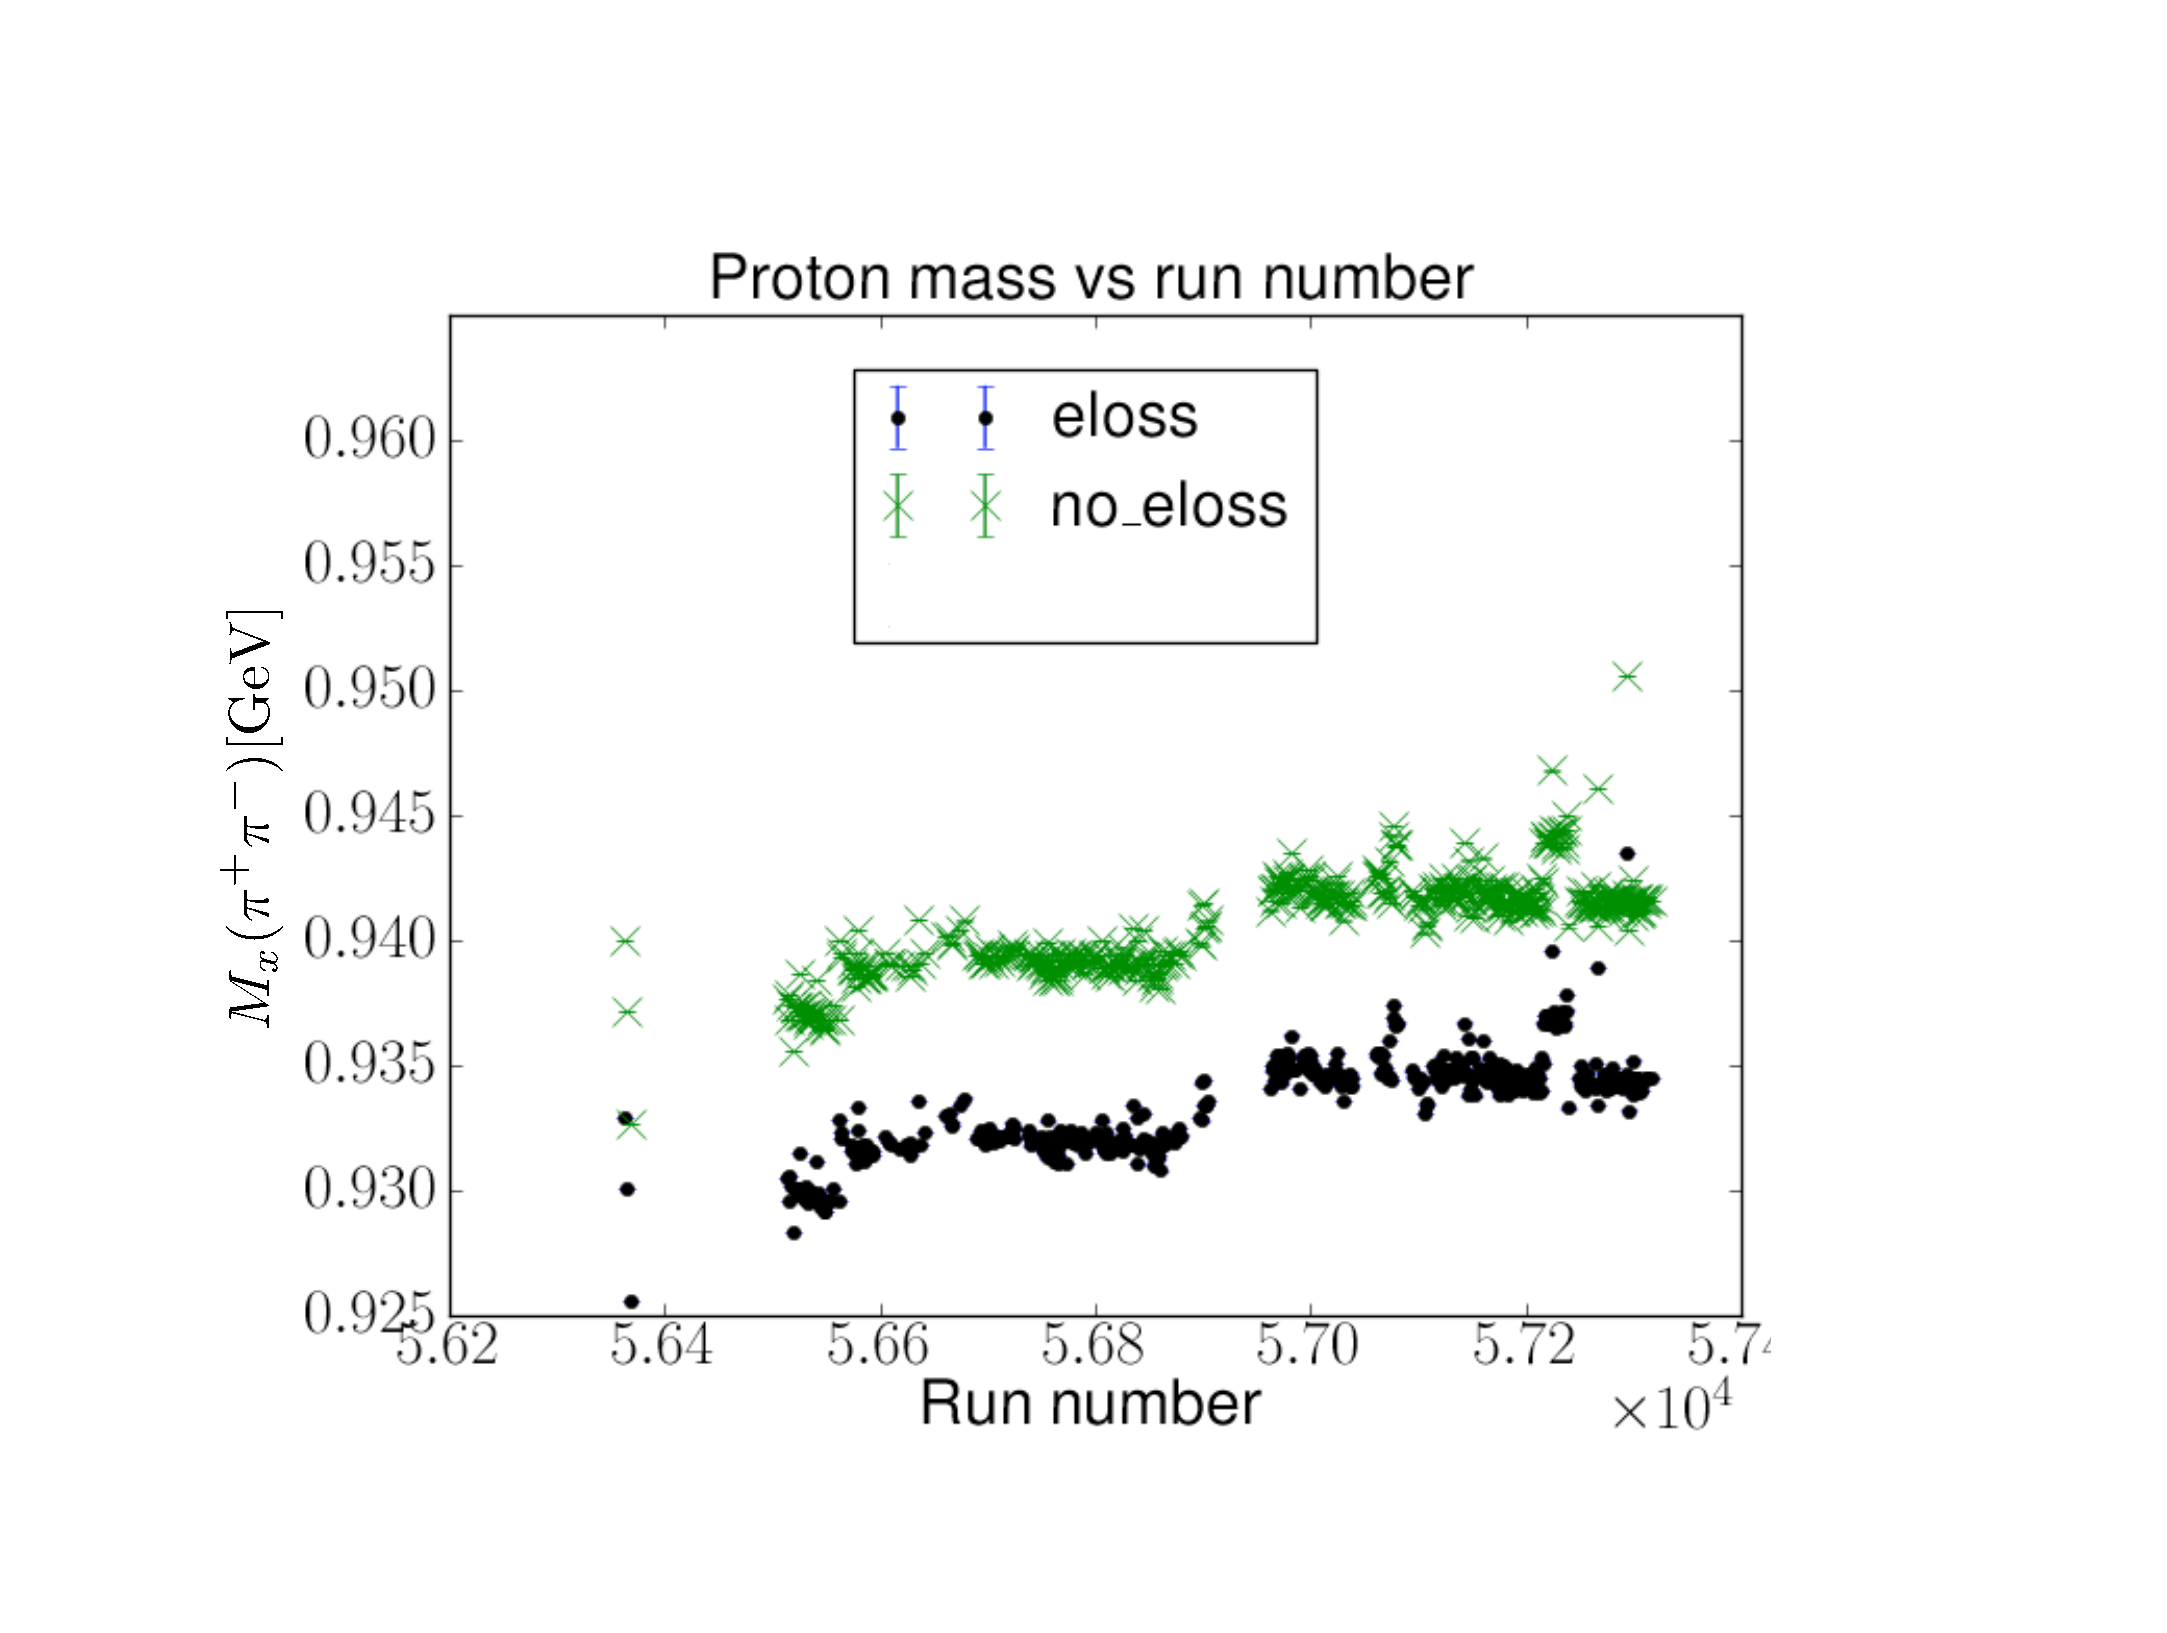
\includegraphics[width=0.6\textwidth]{figures/calib/tag/ecor/P_mass_issue.eps}
\caption[Run Number vs. Proton Mass ]{\label{fig:beamcor.p_mass}Plot of \desg{g12} run number vs. proton mass with and without the ``energy-loss'' applied. \abbr{PDG} mass for the proton is 0.938272 GeV/c. }
\end{center}\end{figure}

\begin{figure}\begin{center}
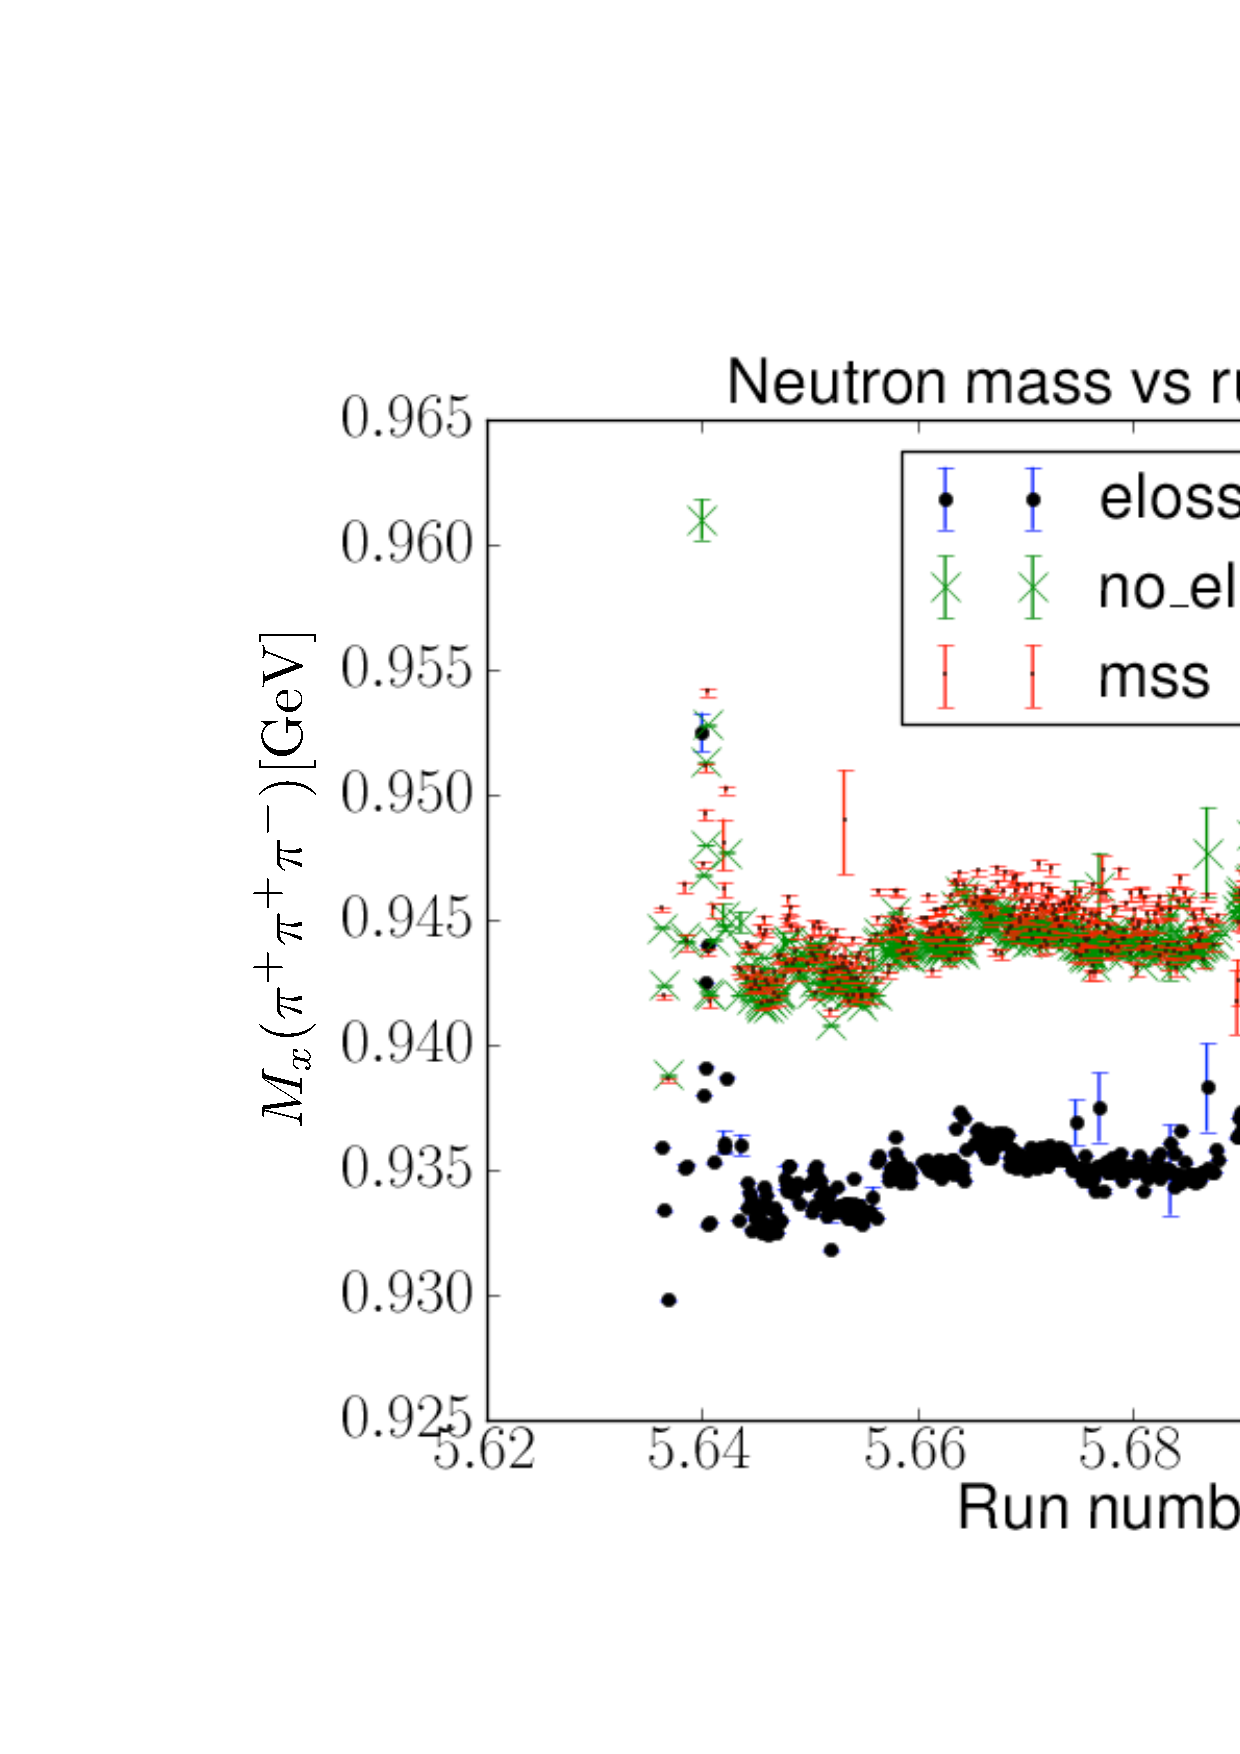
\includegraphics[width=0.6\textwidth]{figures/calib/tag/ecor/N_mass_issue.pdf}
\caption[Run Number vs. Neutron Mass]{\label{fig:beamcor.n_mass}Plot of \desg{g12} run number vs. neutron mass with and without the ``energy-loss'' applied. \abbr{PDG} mass for the neutron is 0.939565 GeV/c. Image Source:~\cite{bookwalter}}
\end{center}\end{figure}

\begin{figure}\begin{center}
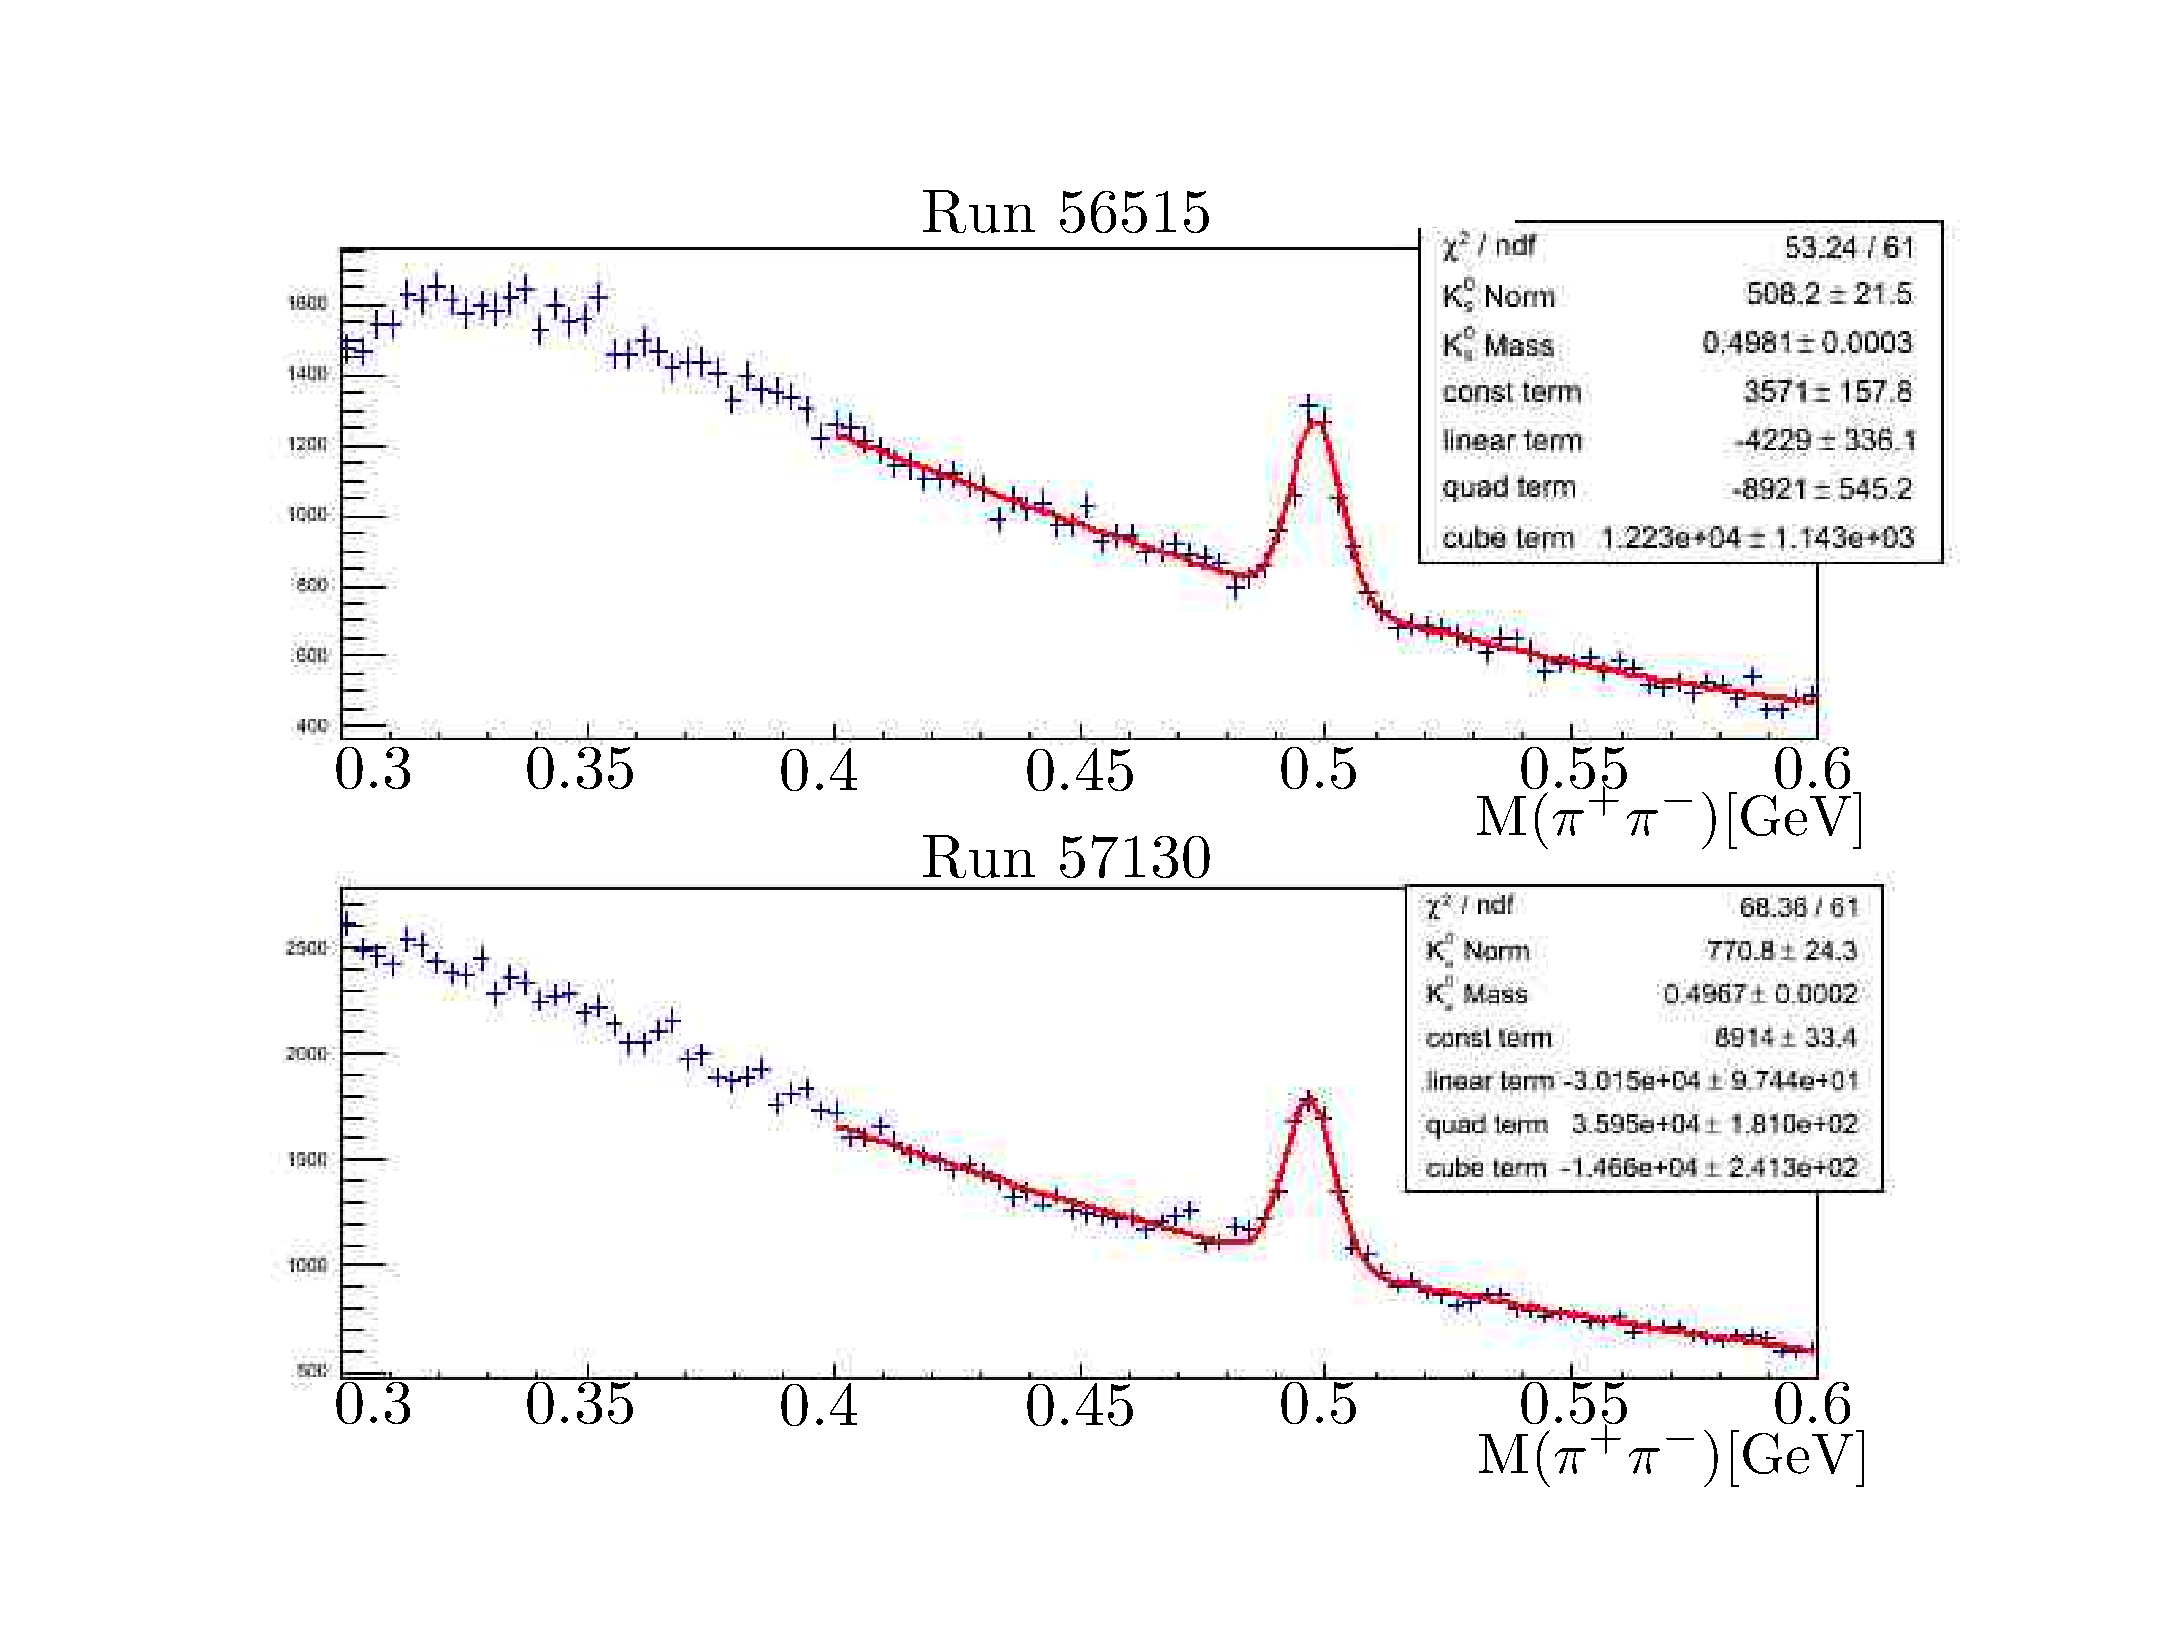
\includegraphics[width=0.6\textwidth]{figures/calib/tag/ecor/Kaon_mass.eps}
\caption[Kaon Mass for Run 56515 and 57130]{\label{fig:beamcor.k_mass}Plot of Kaon mass for runs 56515 and 57130.  \abbr{PDG} mass for the kaon is 0.497614 GeV/c.}
\end{center}\end{figure}

\FloatBarrier

Now that it is known that the photon beam energy is the cause of the issue, it must be known the cause of the photon beam error. Several quantities that the tagger subsystem are subjected to were analyzed, first being the tagger magnet current which, according to the \abbr{EPICS} Fig~\ref{fig:tag.magnet.epics}, remain constant
but showed that around run = 56920 (May 12, 2008) the tagger magnet was shut-off. The tagger magnet shut-off was done because work had to be done in the hall, however after the tagger magnet was turned on, the current was set to its previous setting. A further investigation into the tagger magnet was performed by private communication with the accelerator group chief Arne Freyberger, Fig~\ref{fig:tag.magnet.arne} shows the data the accelerator group had for the tagger magnet which confirms that the tagger magnet current was stable throughout the running of \desg{g12}. The next beam quantity analyzed was the beam current delivered by \abbr{CEBAF}, again through private communication with the accelerator group chief Arne Freyberger it is shown in Fig.~\ref{fig:beamcurrents} that the electron beam current remained constant throughout the \desg{g12} experiment.
\begin{figure}\begin{center}
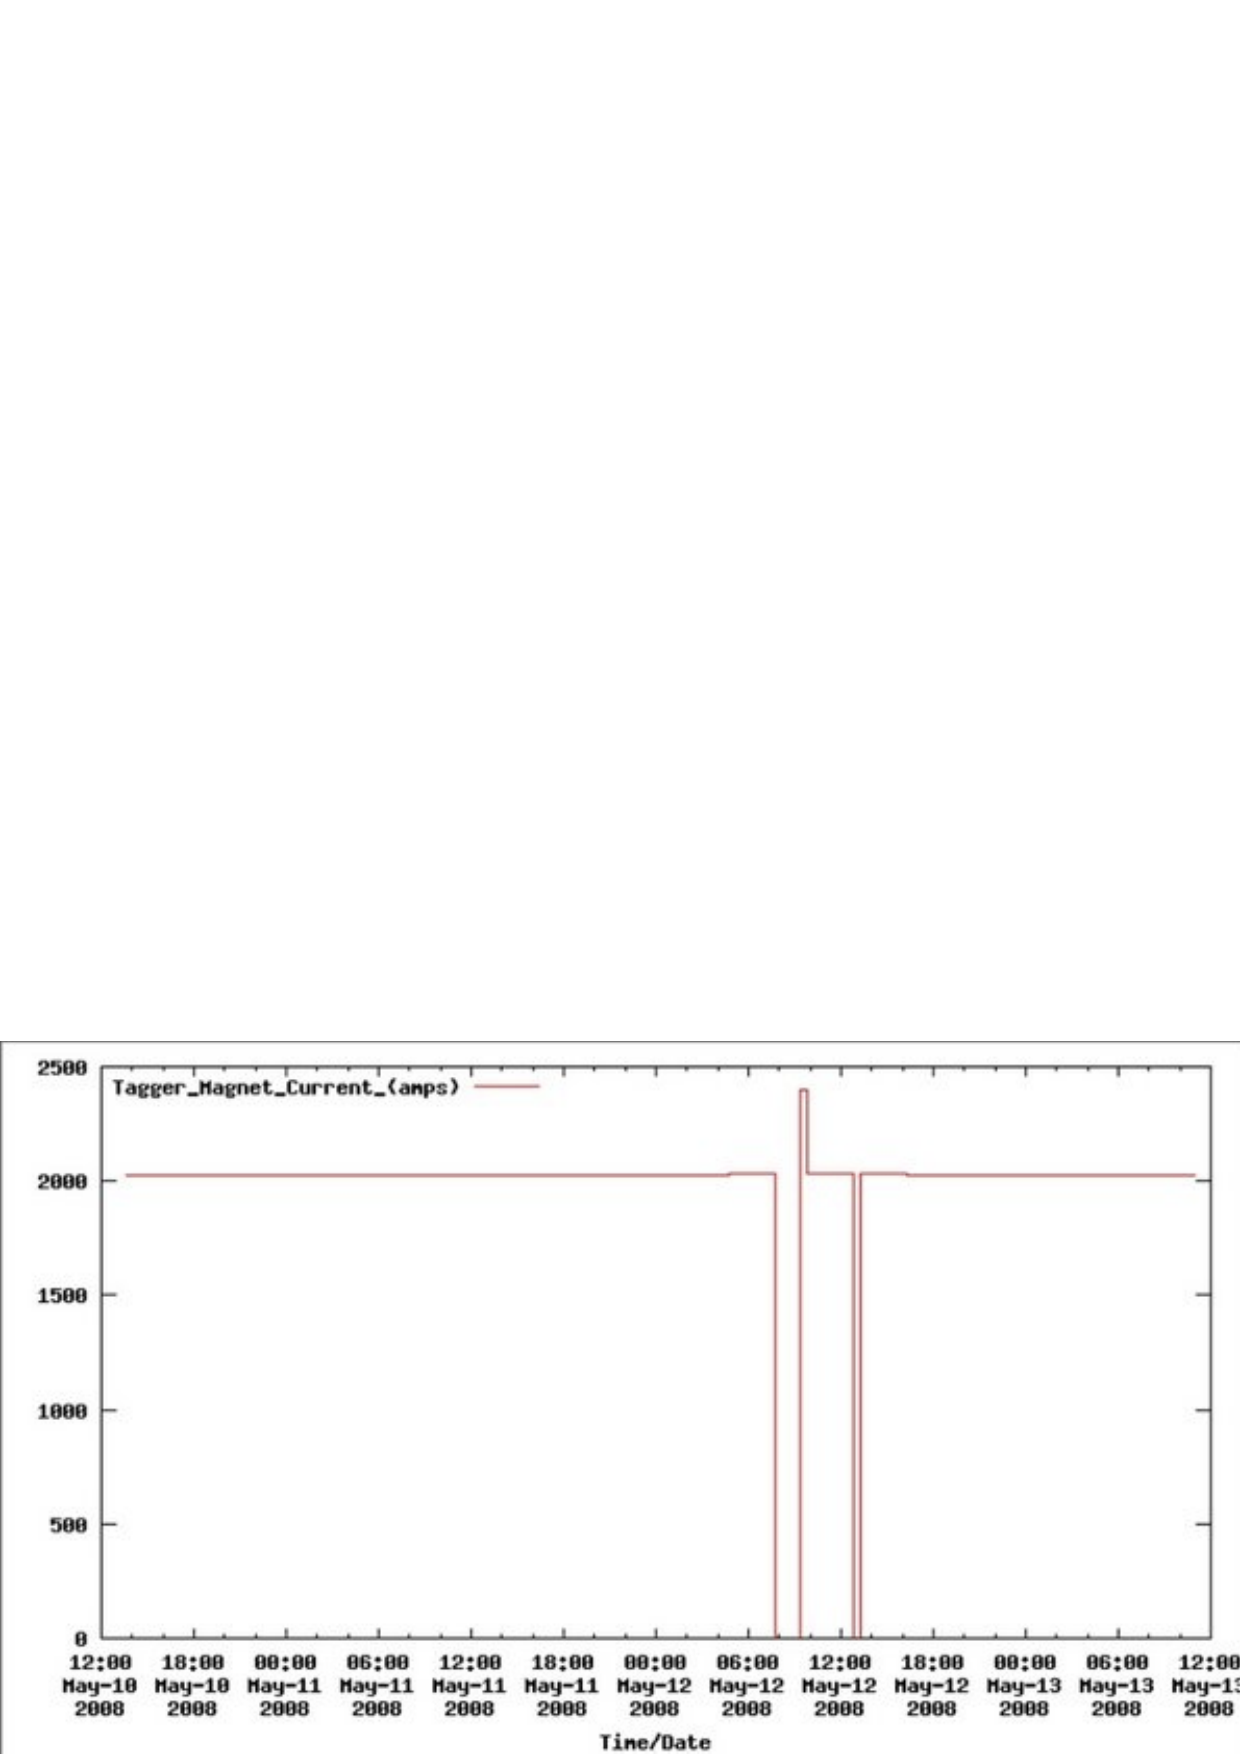
\includegraphics[width=0.6\textwidth]{figures/calib/tag/ecor/600px-Hystersis_smokingGun.pdf}
\caption[Current of Tagger Magnet from \abbr{EPICS}]{\label{fig:tag.magnet.epics}Tagger magnet current according to \abbr{EPICS}}
\end{center}\end{figure}

\begin{figure}\begin{center}
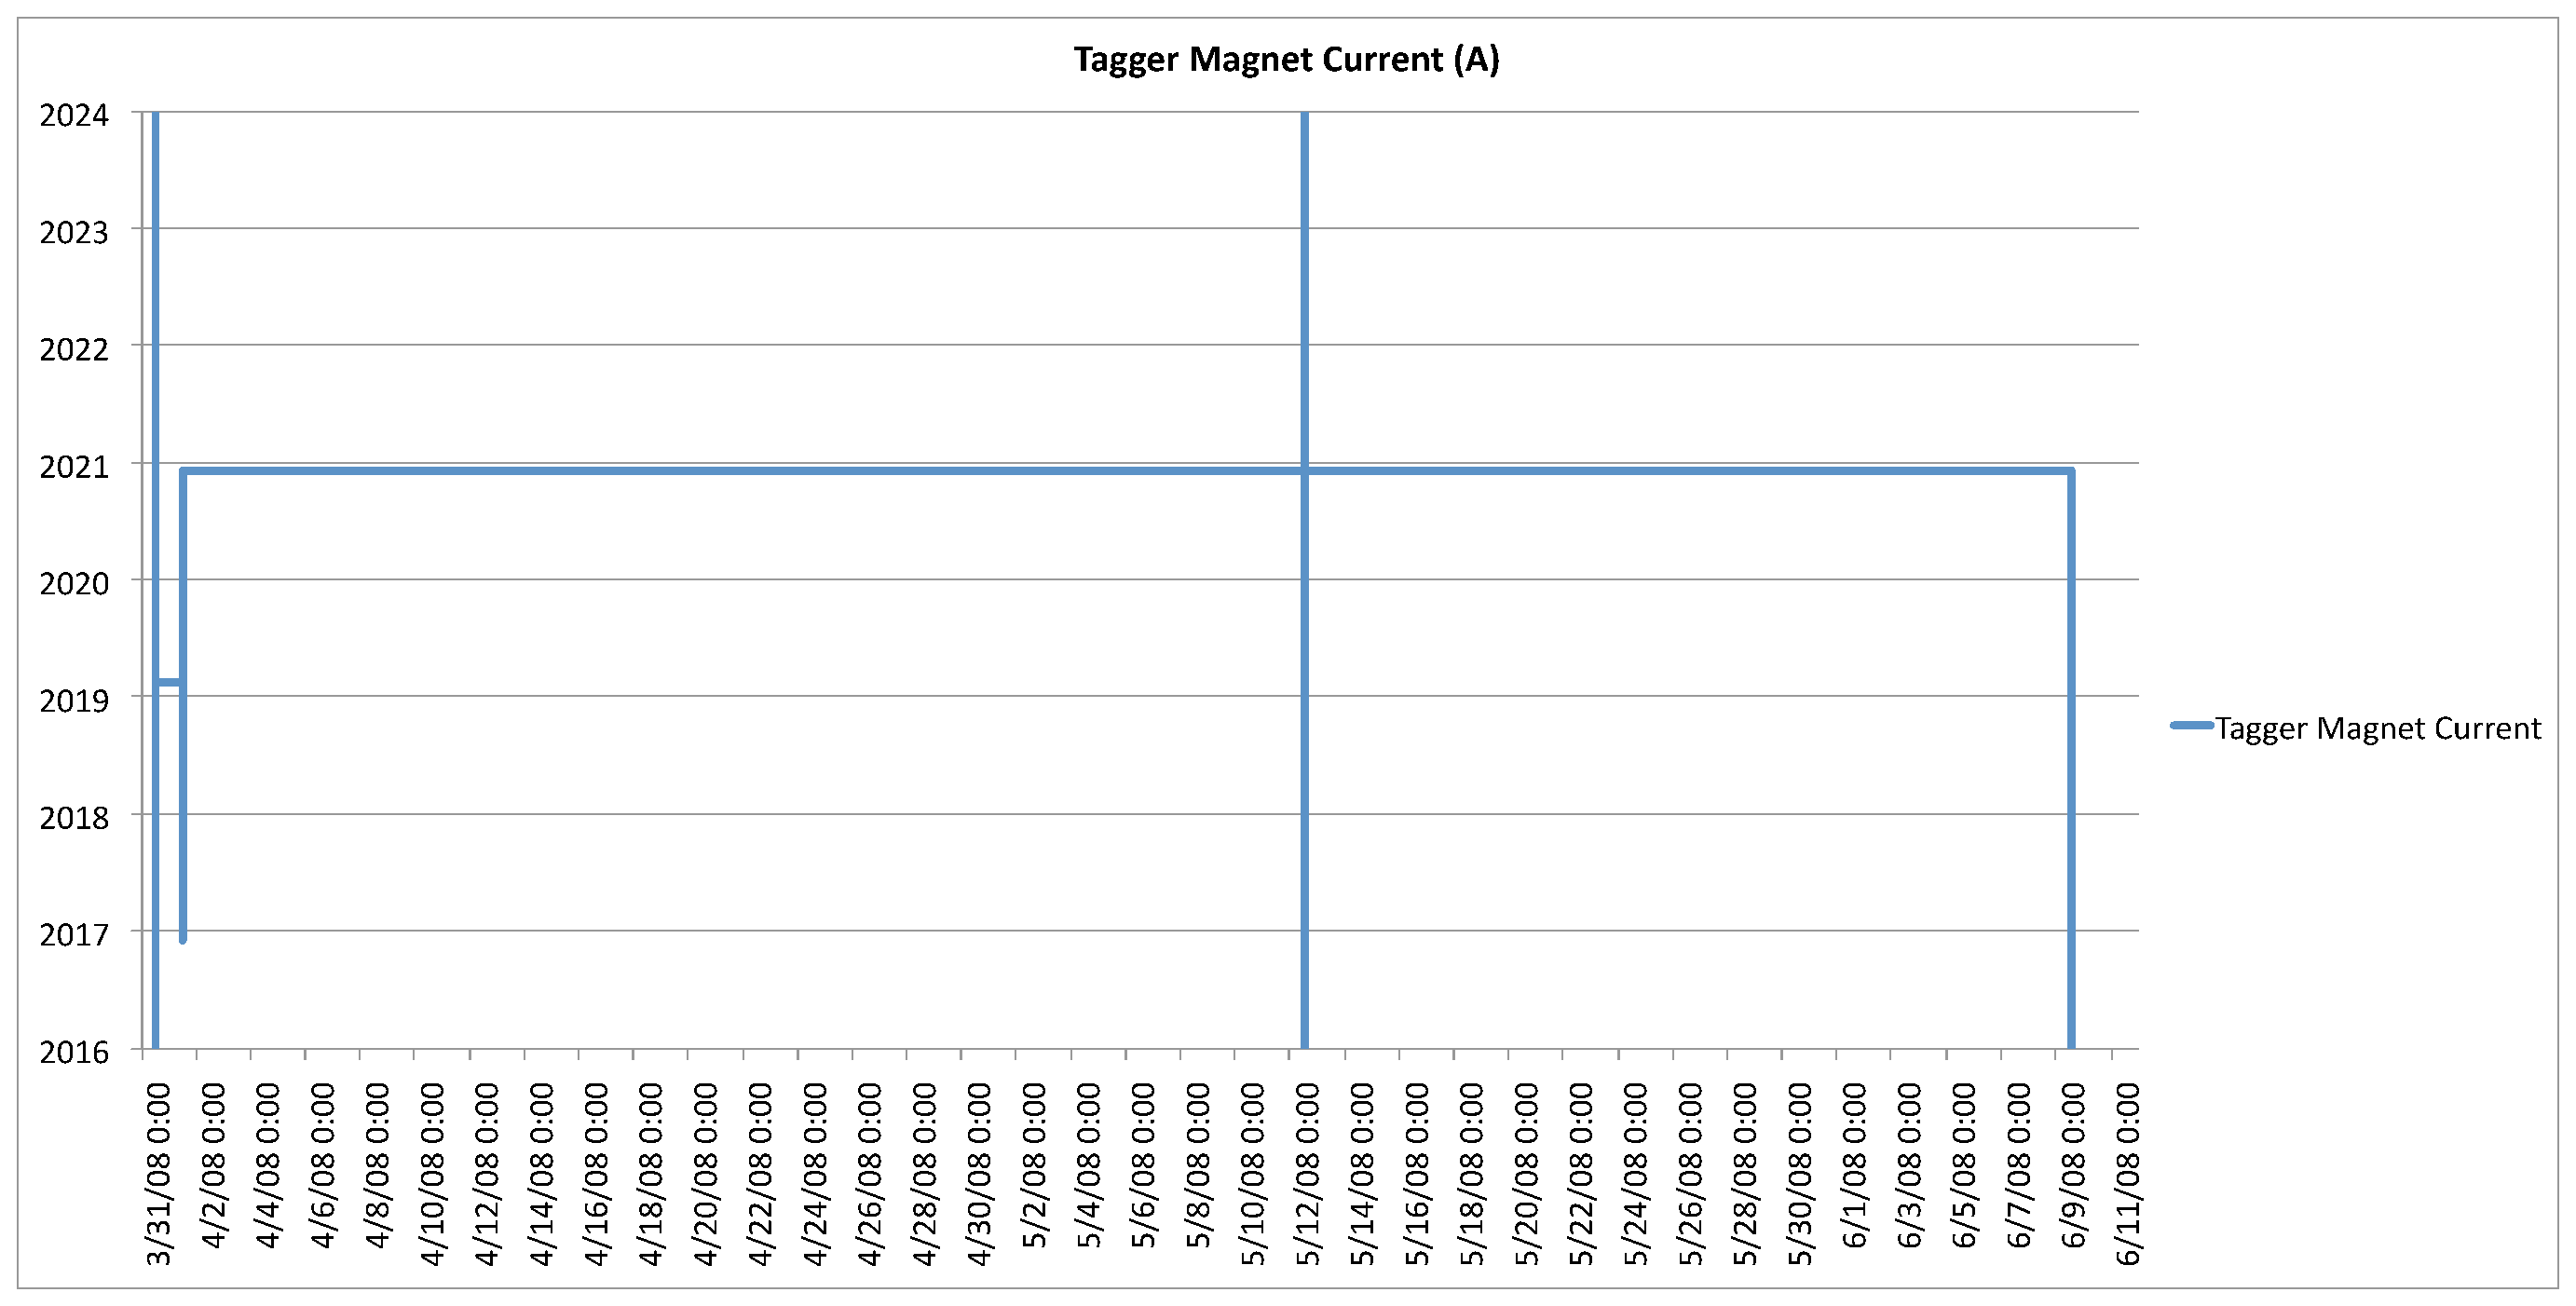
\includegraphics[width=0.6\textwidth]{figures/calib/tag/ecor/tagger_current_arne.eps}
\caption[Current of Tagger Magnet from Accelerator Group]{\label{fig:tag.magnet.arne} Tagger magnet current according to accelerator group}
\end{center}\end{figure}

\begin{figure}\begin{center}
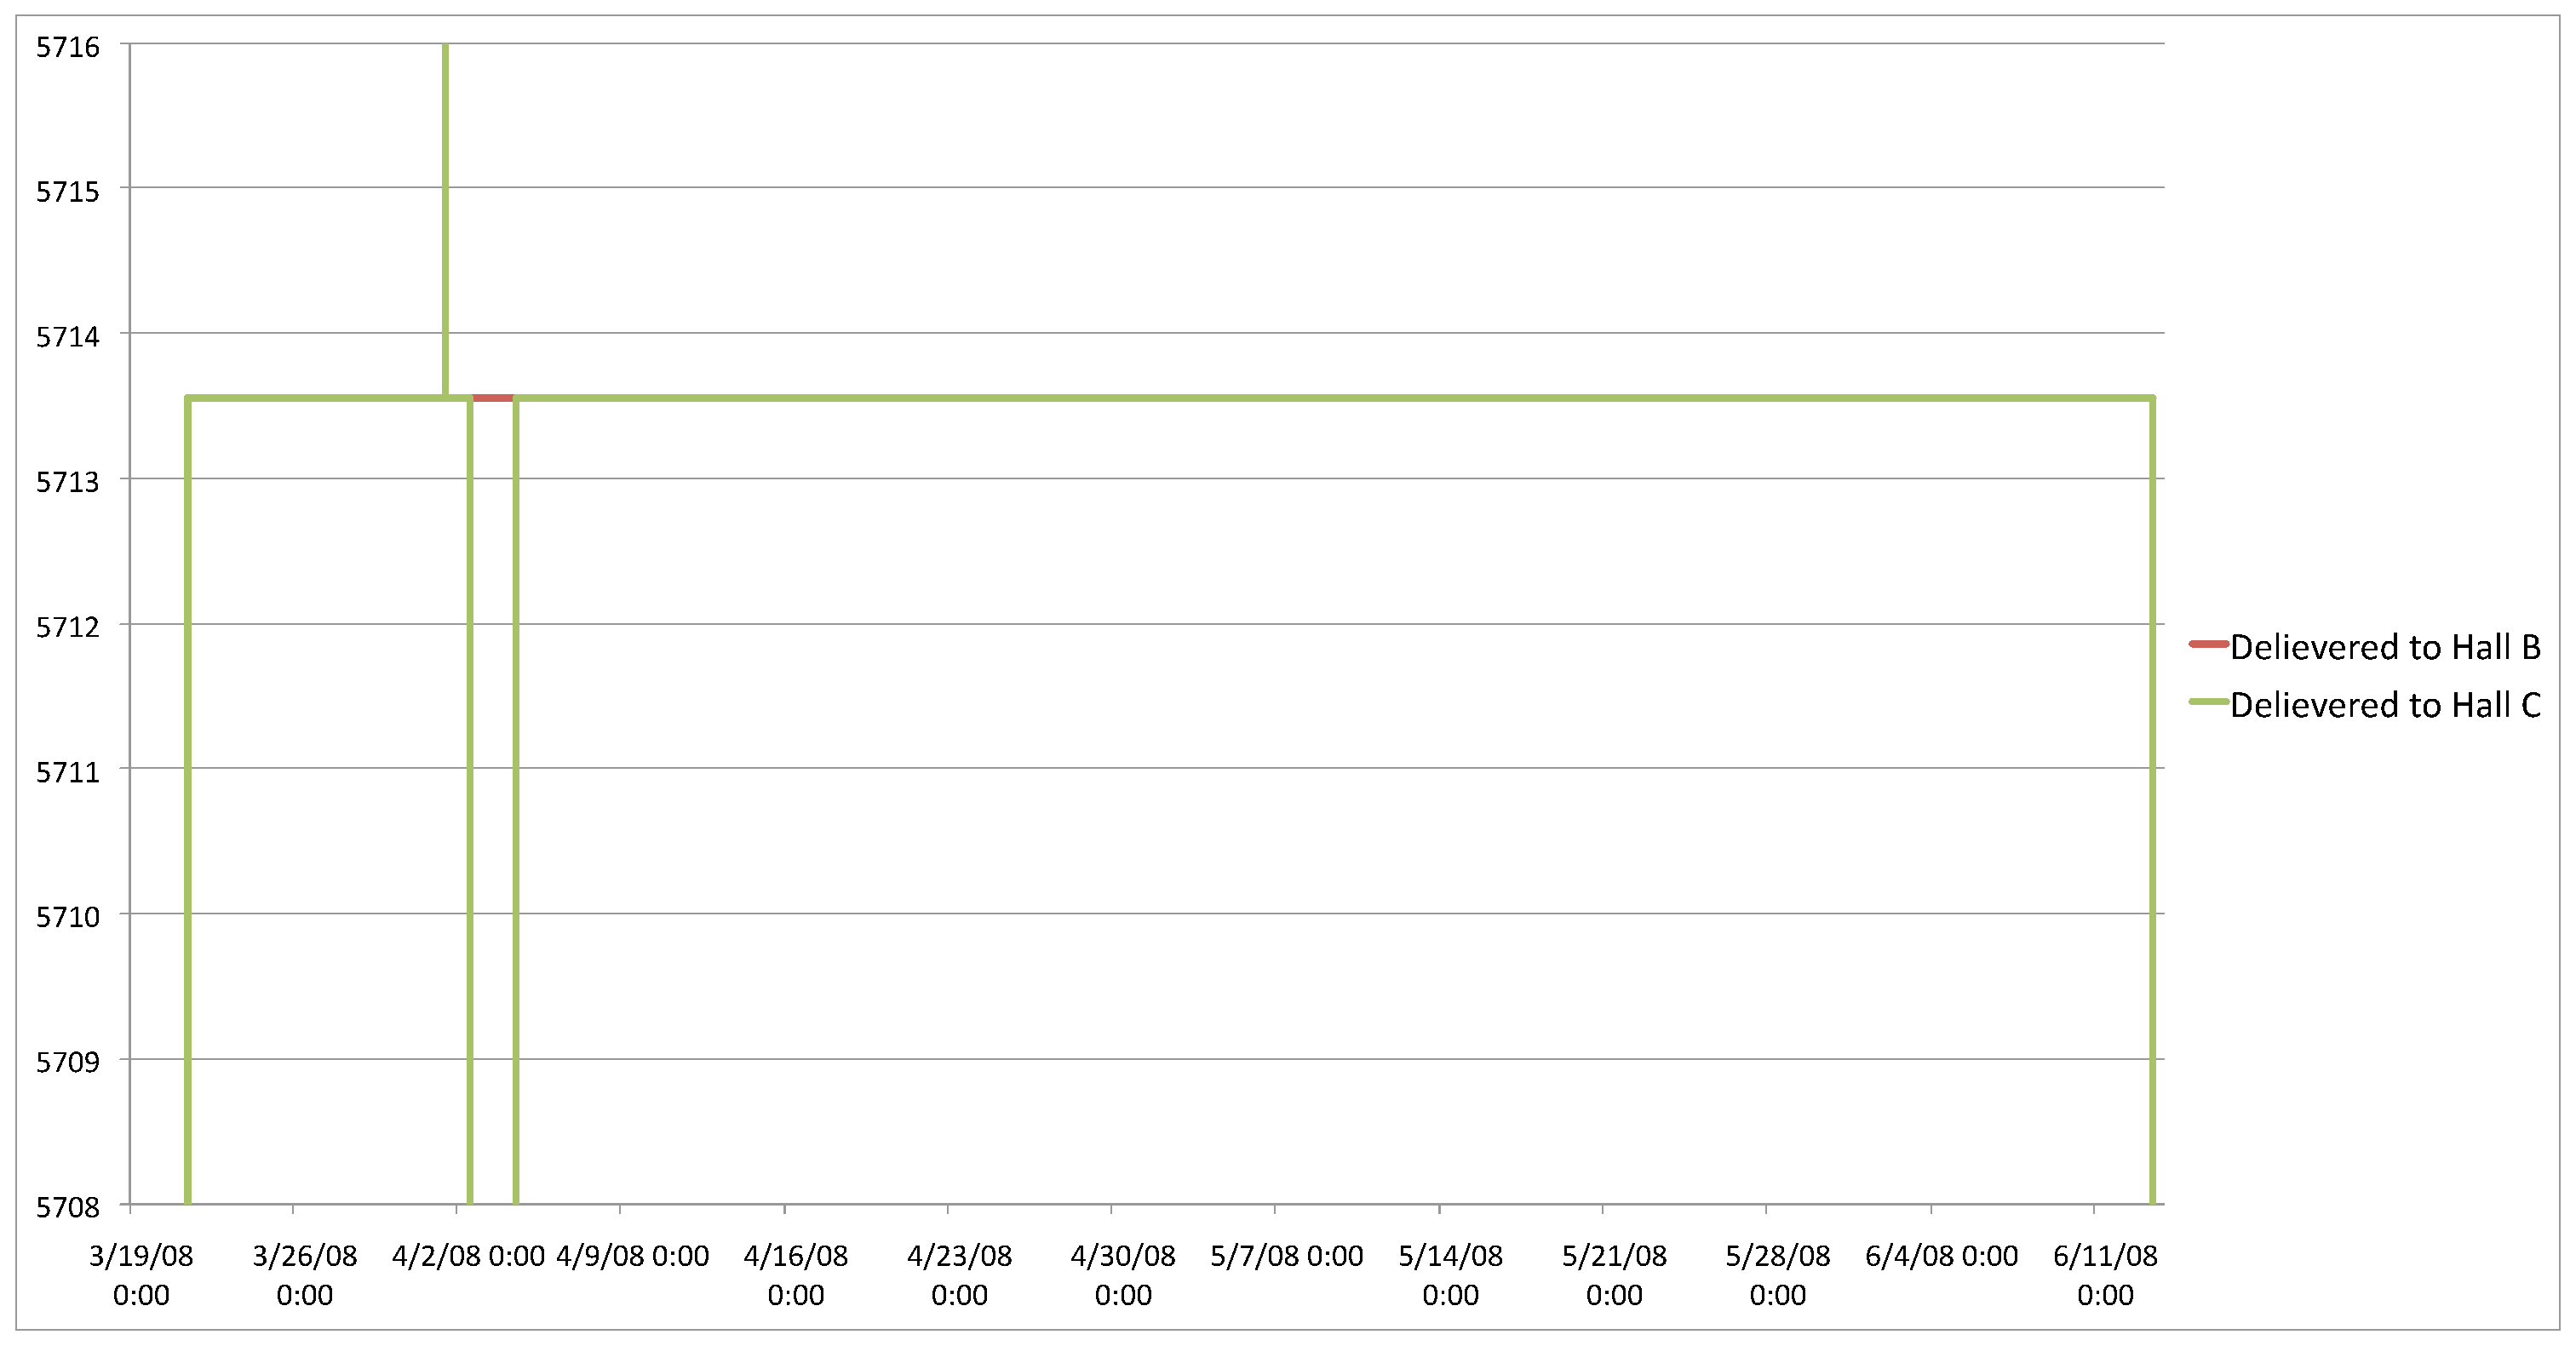
\includegraphics[width=0.6\textwidth]{figures/calib/tag/ecor/beam_currentsII.eps}
\caption[Electron Beam Current Delivered to hall \desg{b} and hall \desg{c} ]{\label{fig:beamcurrents}Electron beam current delivered to hall \desg{b}(red) and hall \desg{c} (green) according to accelerator group during the time of \desg{g12} running }
\end{center}\end{figure}

The next quantity investigated was the positioning of the tagger dump. This quantity was used in place of the tagger magnetic field strength because hall \desg{b} does not measure the tagger magnetic field strength, however since the radius of curvature a charged particle travels is proportional to the magnetic field, Eq.~\ref{eq:motioninmagII}, this quantity is suitable.
\begin{equation}\label{eq:motioninmagII}
    p = q(v \times B)r
\end{equation}
The y-positioning of the tagger dump jumps on or about May 12, 2008, Fig.~\ref{fig:tagdump}. This would effect how the tagger recorded the scattered electron. A cause for the change in y-positioning can only be due to the magnetic field changing. The phenomena in magnetism that allows for a steady current but a change in magnetic field is known as hysteresis, Fig.~\ref{fig:hyst} illustrates that on the x-axis there is a constant current that is associated with 2 distinct magnetic fields shown on the y-axis of Fig.~\ref{fig:hyst}.
\begin{figure}\begin{center}
\includegraphics[width=0.6\textwidth]{figures/calib/tag/ecor/600px-Tagger-dump-y.pdf}
\caption[Tagger Dump Y-Positioning]{\label{fig:tagdump}Tagger dump y-positioning according to \abbr{EPICS}}
\end{center}\end{figure}

\begin{figure}\begin{center}
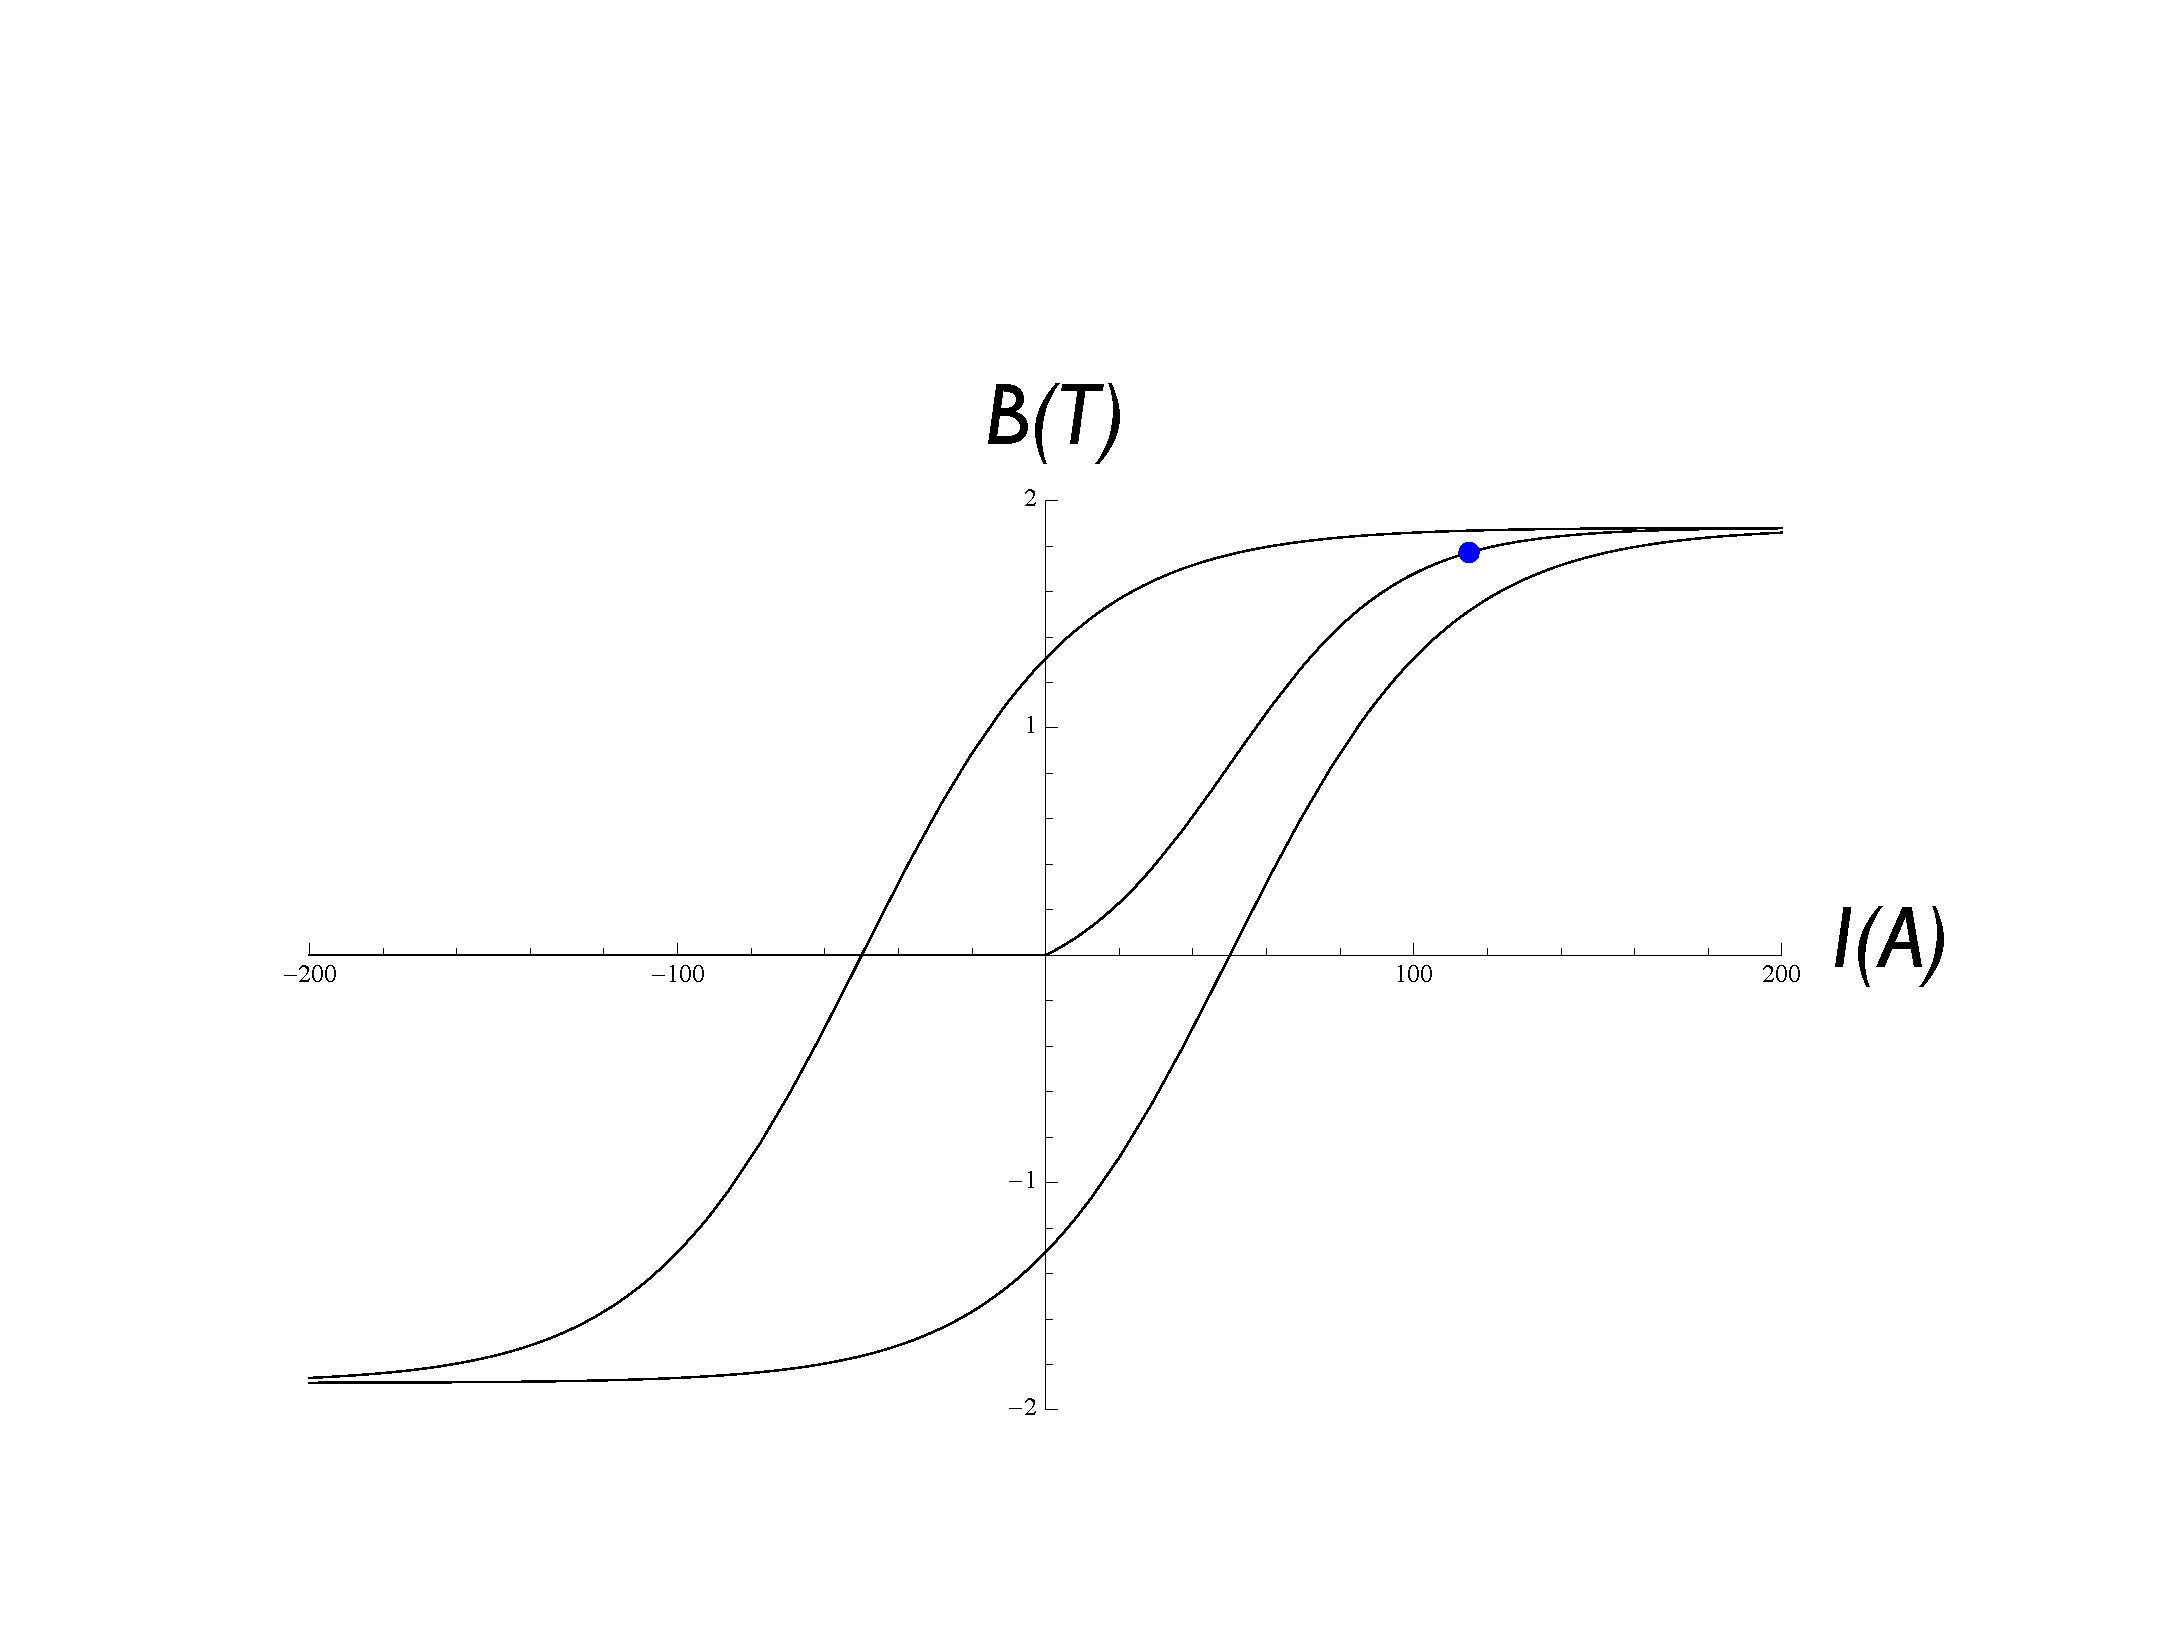
\includegraphics[width=0.6\textwidth]{figures/calib/tag/ecor/hysteresis_keynote.eps}
\caption[Plot Depicting the Process of Hysteresis]{\label{fig:hyst}Plot depicting the process of hysteresis. For the a current of strength I, there could exist two magnetic fields of strength B. Image source:~\cite{clas.thesis.kunkel}}
\end{center}\end{figure}
\FloatBarrier
Now that it is determined that the cause of the \desg{g12} missing mass fluctuations are due to hysteresis and the effect would be on the scarred electron, the \desg{g12} data stream was corrected in the following manner. Lets let
\begin{align}
P_\text{π$^+$} + P_\text{π$^-$} = P_\text{π$^+$ π$^-$} \nonumber
\end{align}
therefore
\begin{align}
&(P_\text{γ} + P_\mathrm{target} - (P_\text{π$^+$π$^-$}))^2 = m_p^2 \\
& P_\text{γ}^2 + P_\mathrm{target}^2 + P_\text{π$^+$π$^-$}^2 + 2P_\text{γ}P_\mathrm{target} - 2P_\text{γ}P_\text{π$^+$π$^-$} - 2P_\mathrm{target}P_\text{π$^+$π$^-$}= m_p^2\\
\end{align}
collecting terms of $P_\text{γ}$ to one side and using $P_\mathrm{target}^2 = m_p^2 $ and $P_\text{γ}^2 = 0$
\begin{align}\label{eq:hyst.eqI}
 P_\text{π$^+$π$^-$}^2 - 2P_\mathrm{target}P_\text{π$^+$π$^-$}= 2P_\text{γ}(P_\text{π$^+$π$^-$} - P_\mathrm{target})
\end{align}
From this using eq.~\ref{eq:tagger.energy} in 4-vector notation
\begin{align}\label{eq:tagger.energyII}
P_\text{γ} = P_{E_0} - P_\text{e}\nonumber
\end{align}
where $P_{E_0}$ is the beam energy delivered from \abbr{CEBAF} as recorded in the \abbr{RUNC} bank and $P_\text{e}$ is the scattered electron in the \emph{bremsstrahlung} process that is recorded by the tagger. From eq.~\ref{eq:tagger.energy} the only known quantities are $P_{E_0}$ and $P_\text{γ}$. Applying a scaler correction to $P_\text{e}$ as $xP_\text{e}$ and solving for $x$ for all known quantities, eq.~\ref{eq:hyst.eqI} simplifies to;
\begin{align}
x= \frac{P_{E_0}(P_\mathrm{target}-P_\text{π$^+$π$^-$}) + P_\text{π$^+$π$^-$}^2/2  - P_\mathrm{target}P_\text{π$^+$π$^-$}}{(P_{E_0} - P_\text{γ})(P_\mathrm{target} - P_\text{π$^+$π$^-$})}
\end{align}
To reduce statistical fluctuations $\frac{1}{10}$ of run 56515 was analyzed to obtain the correction factor $x$. The correction factor was fitted to a $3^\mathrm{rd}$ order polynomial $\pm~0.008$ from the mean of the peak to establish an accurate measurement of the peak, this is shown in Fig~\ref{fig:56515.cor}. After the correction factor was extracted for run 56515, it was applied to both the topologies listed in Eq.~\ref{eq:beam.cortopology} and Eq.~\ref{eq:beam.checktopology} by recalculating the photon beam energy as;
\begin{align}
E_e = E_{\abbr{CEBAF}} - E_{γ} \nonumber \\
E_{γ}^{new} = E_{E_0} - E_e*x \nonumber.
\end{align}
Figures~\ref{fig:proton.fix},~\ref{fig:neutron.fix} illustrate the missing mass topologies after beam correction and shows that the new calculated missing mass is less than 1~MeV from \abbr{PDG} values. Since both the missing proton mass and missing neutron mass were adjusted properly to the correct mass by using the same beam correction factor, it shows that the correction factor is independent of topology and therefore must be applied to all \desg{g12} analyses. The procedure to calculate $x$ was repeated for every run in \desg{g12}, Fig~\ref{fig:beamcor.run}, with $\frac{1}{10}$ of the data used. To validate the corrections of the entire \desg{g12} data set, the missing neutron mass was recalculated for each run, shown in  Fig.~\ref{fig:neutron.fixall}, using several correction schemes, i.e. a scheme of just ``energy-loss'' corrections, a scheme of ``energy-loss'' and momentum corrections (JTG PCor), a scheme of ``energy-loss'', momentum corrections (JTG PCor) and beam corrections (MK BeamCor) and a scheme of ``energy-loss'' and beam corrections (MK BeamCor). It can be seen in Fig.~\ref{fig:neutron.fixall} that the only scheme that sufficed was the combination of ``energy-loss'' and beam corrections.


\begin{figure}\begin{center}
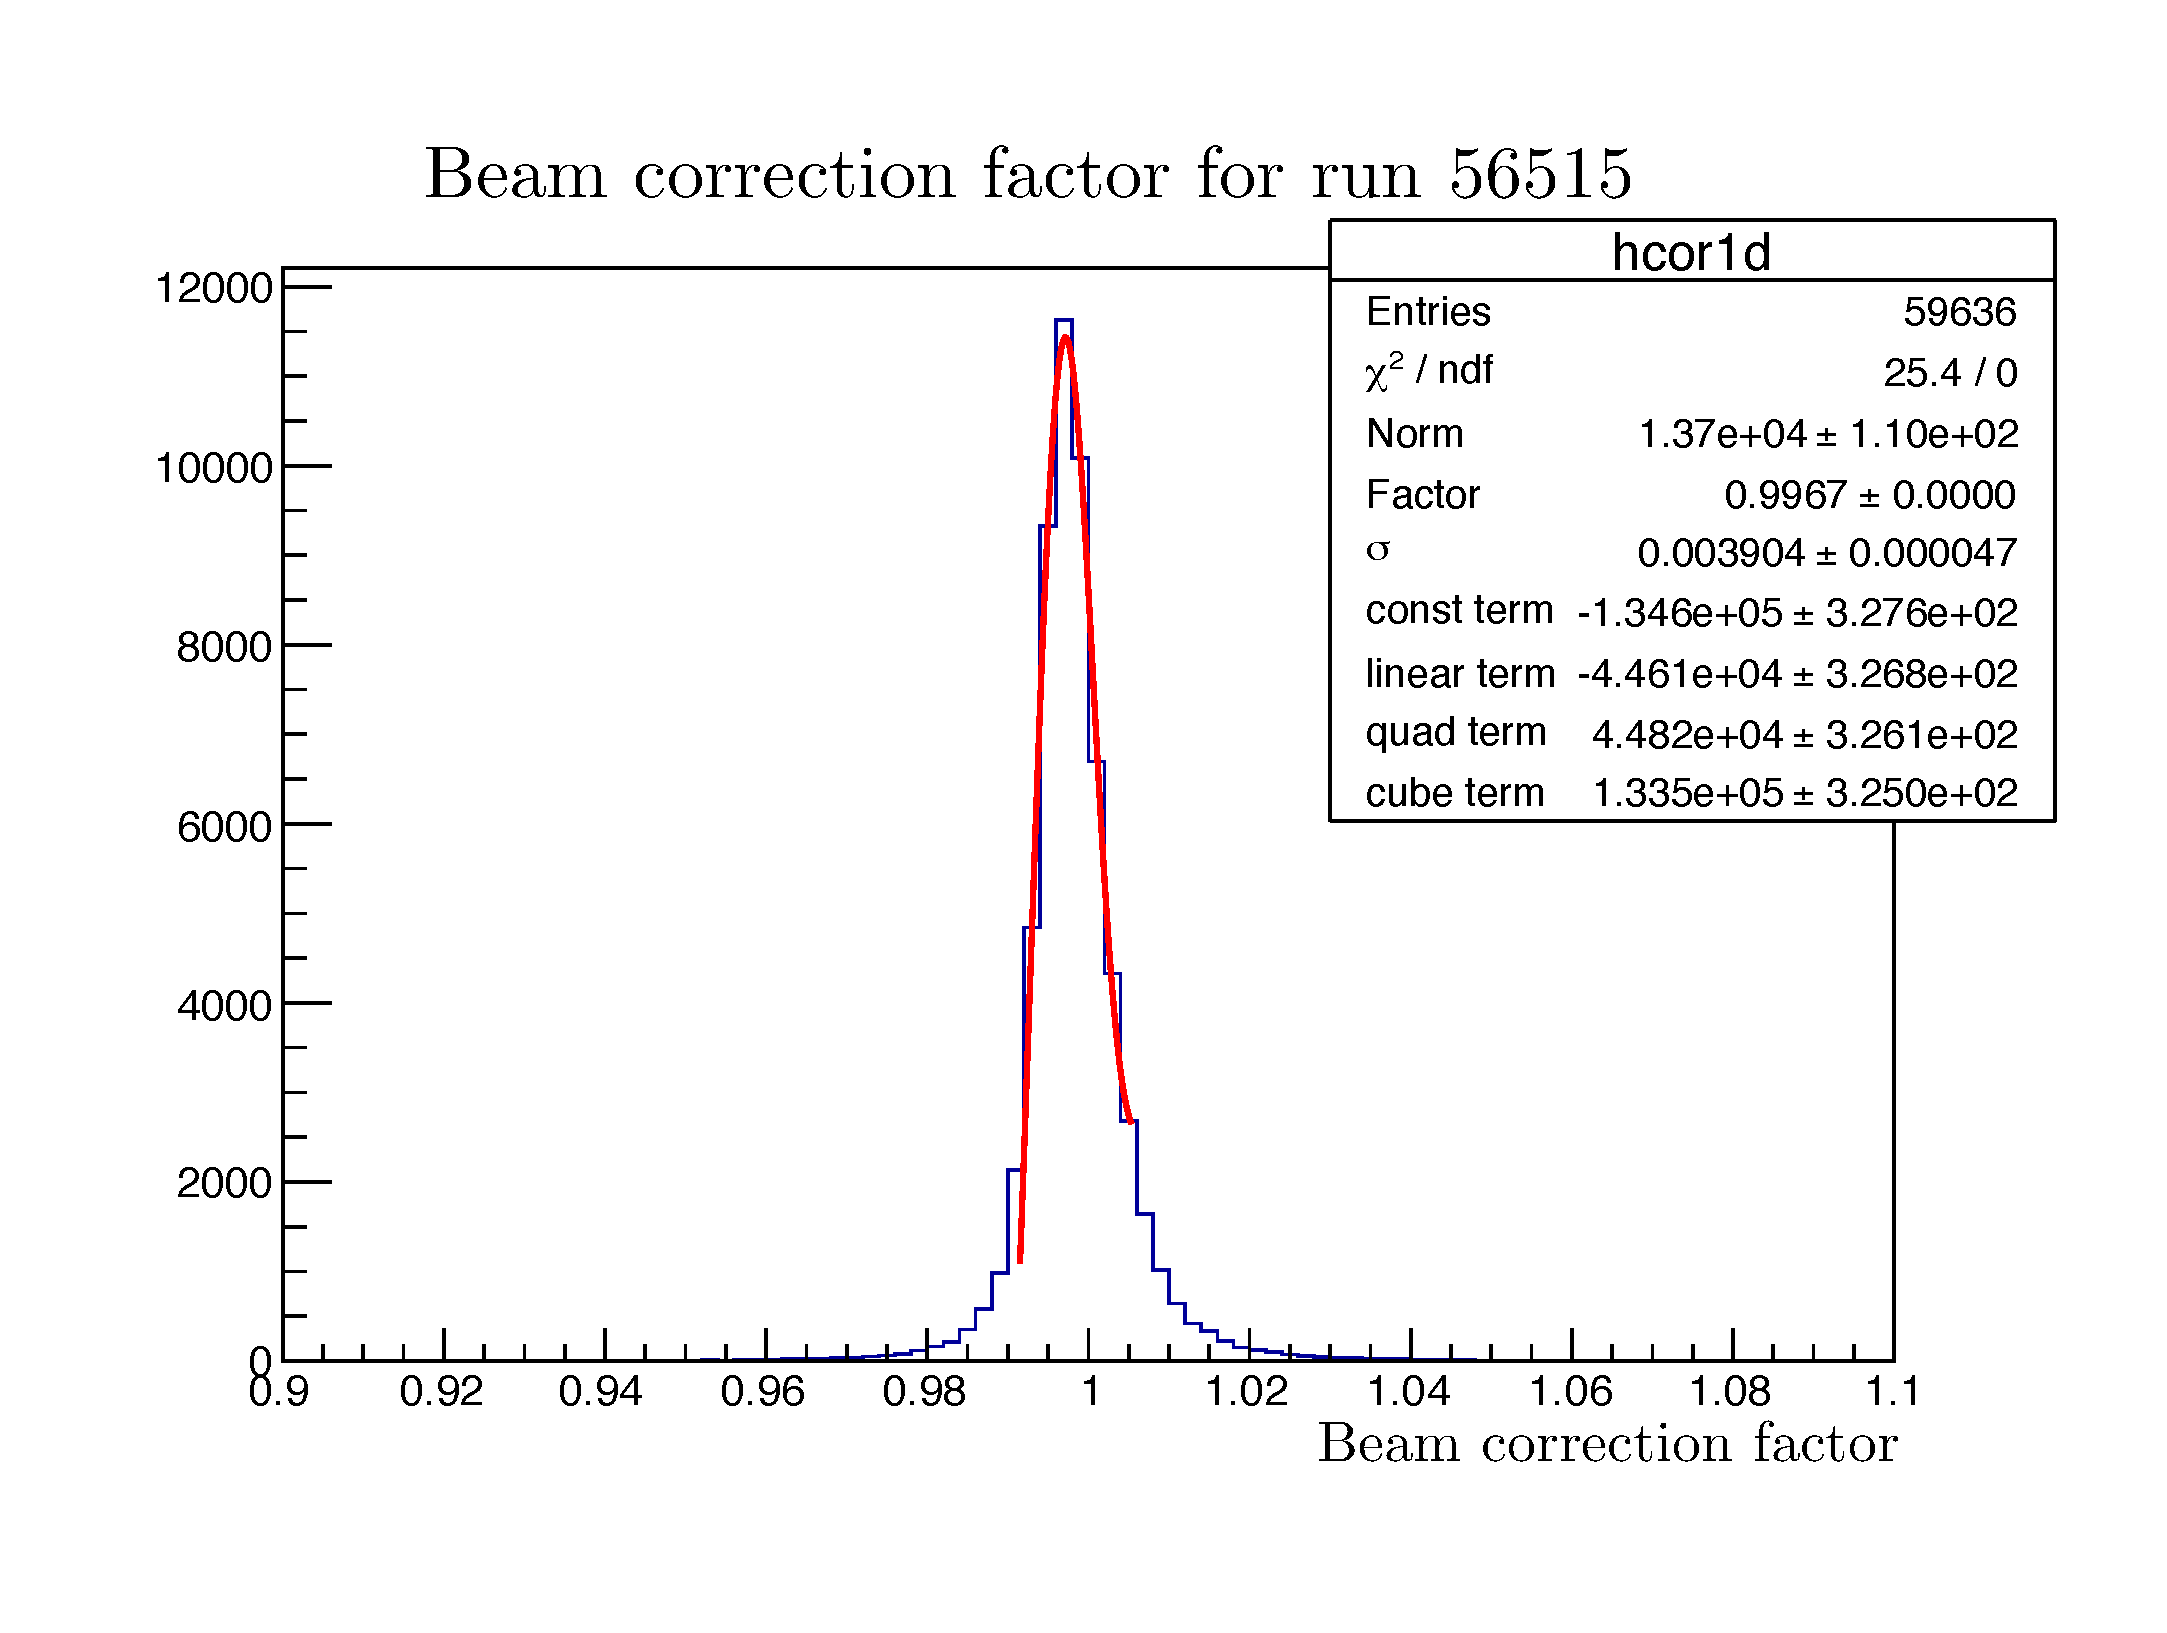
\includegraphics[width=0.6\textwidth]{figures/calib/tag/ecor/56515_cor.eps}
\caption[Beam Correction Factor for Run 56515]{\label{fig:56515.cor} Beam correction factor for run 56515. The fit is a $3^\mathrm{rd}$ order polynomial $\pm~0.008$ from the mean of the peak. Image source:~\cite{clas.thesis.kunkel}}
\end{center}\end{figure}

\begin{figure}\begin{center}
\includegraphics[width=0.6\textwidth]{figures/calib/tag/ecor/FixedmisssingmassII.pdf}
\caption[Proton Mass for Run 56515 After Beam Correction]{\label{fig:proton.fix} Plot of proton mass for runs 56515 after beam correction was applied.  \abbr{PDG} mass for the proton is 0.938272 GeV/c. Image source:~\cite{clas.thesis.kunkel}}
\end{center}\end{figure}

\begin{figure}\begin{center}
\includegraphics[width=0.6\textwidth]{figures/calib/tag/ecor/FixedmisssingmassneutronII.pdf}
\caption[Neutron Mass for Run 56515 After Beam Correction]{\label{fig:neutron.fix} Plot of neutron mass for runs 56515 after beam correction was applied  \abbr{PDG} mass for the neutron is 0.939565 GeV/c. Image source:~\cite{clas.thesis.kunkel}}
\end{center}\end{figure}

\begin{figure}\begin{center}
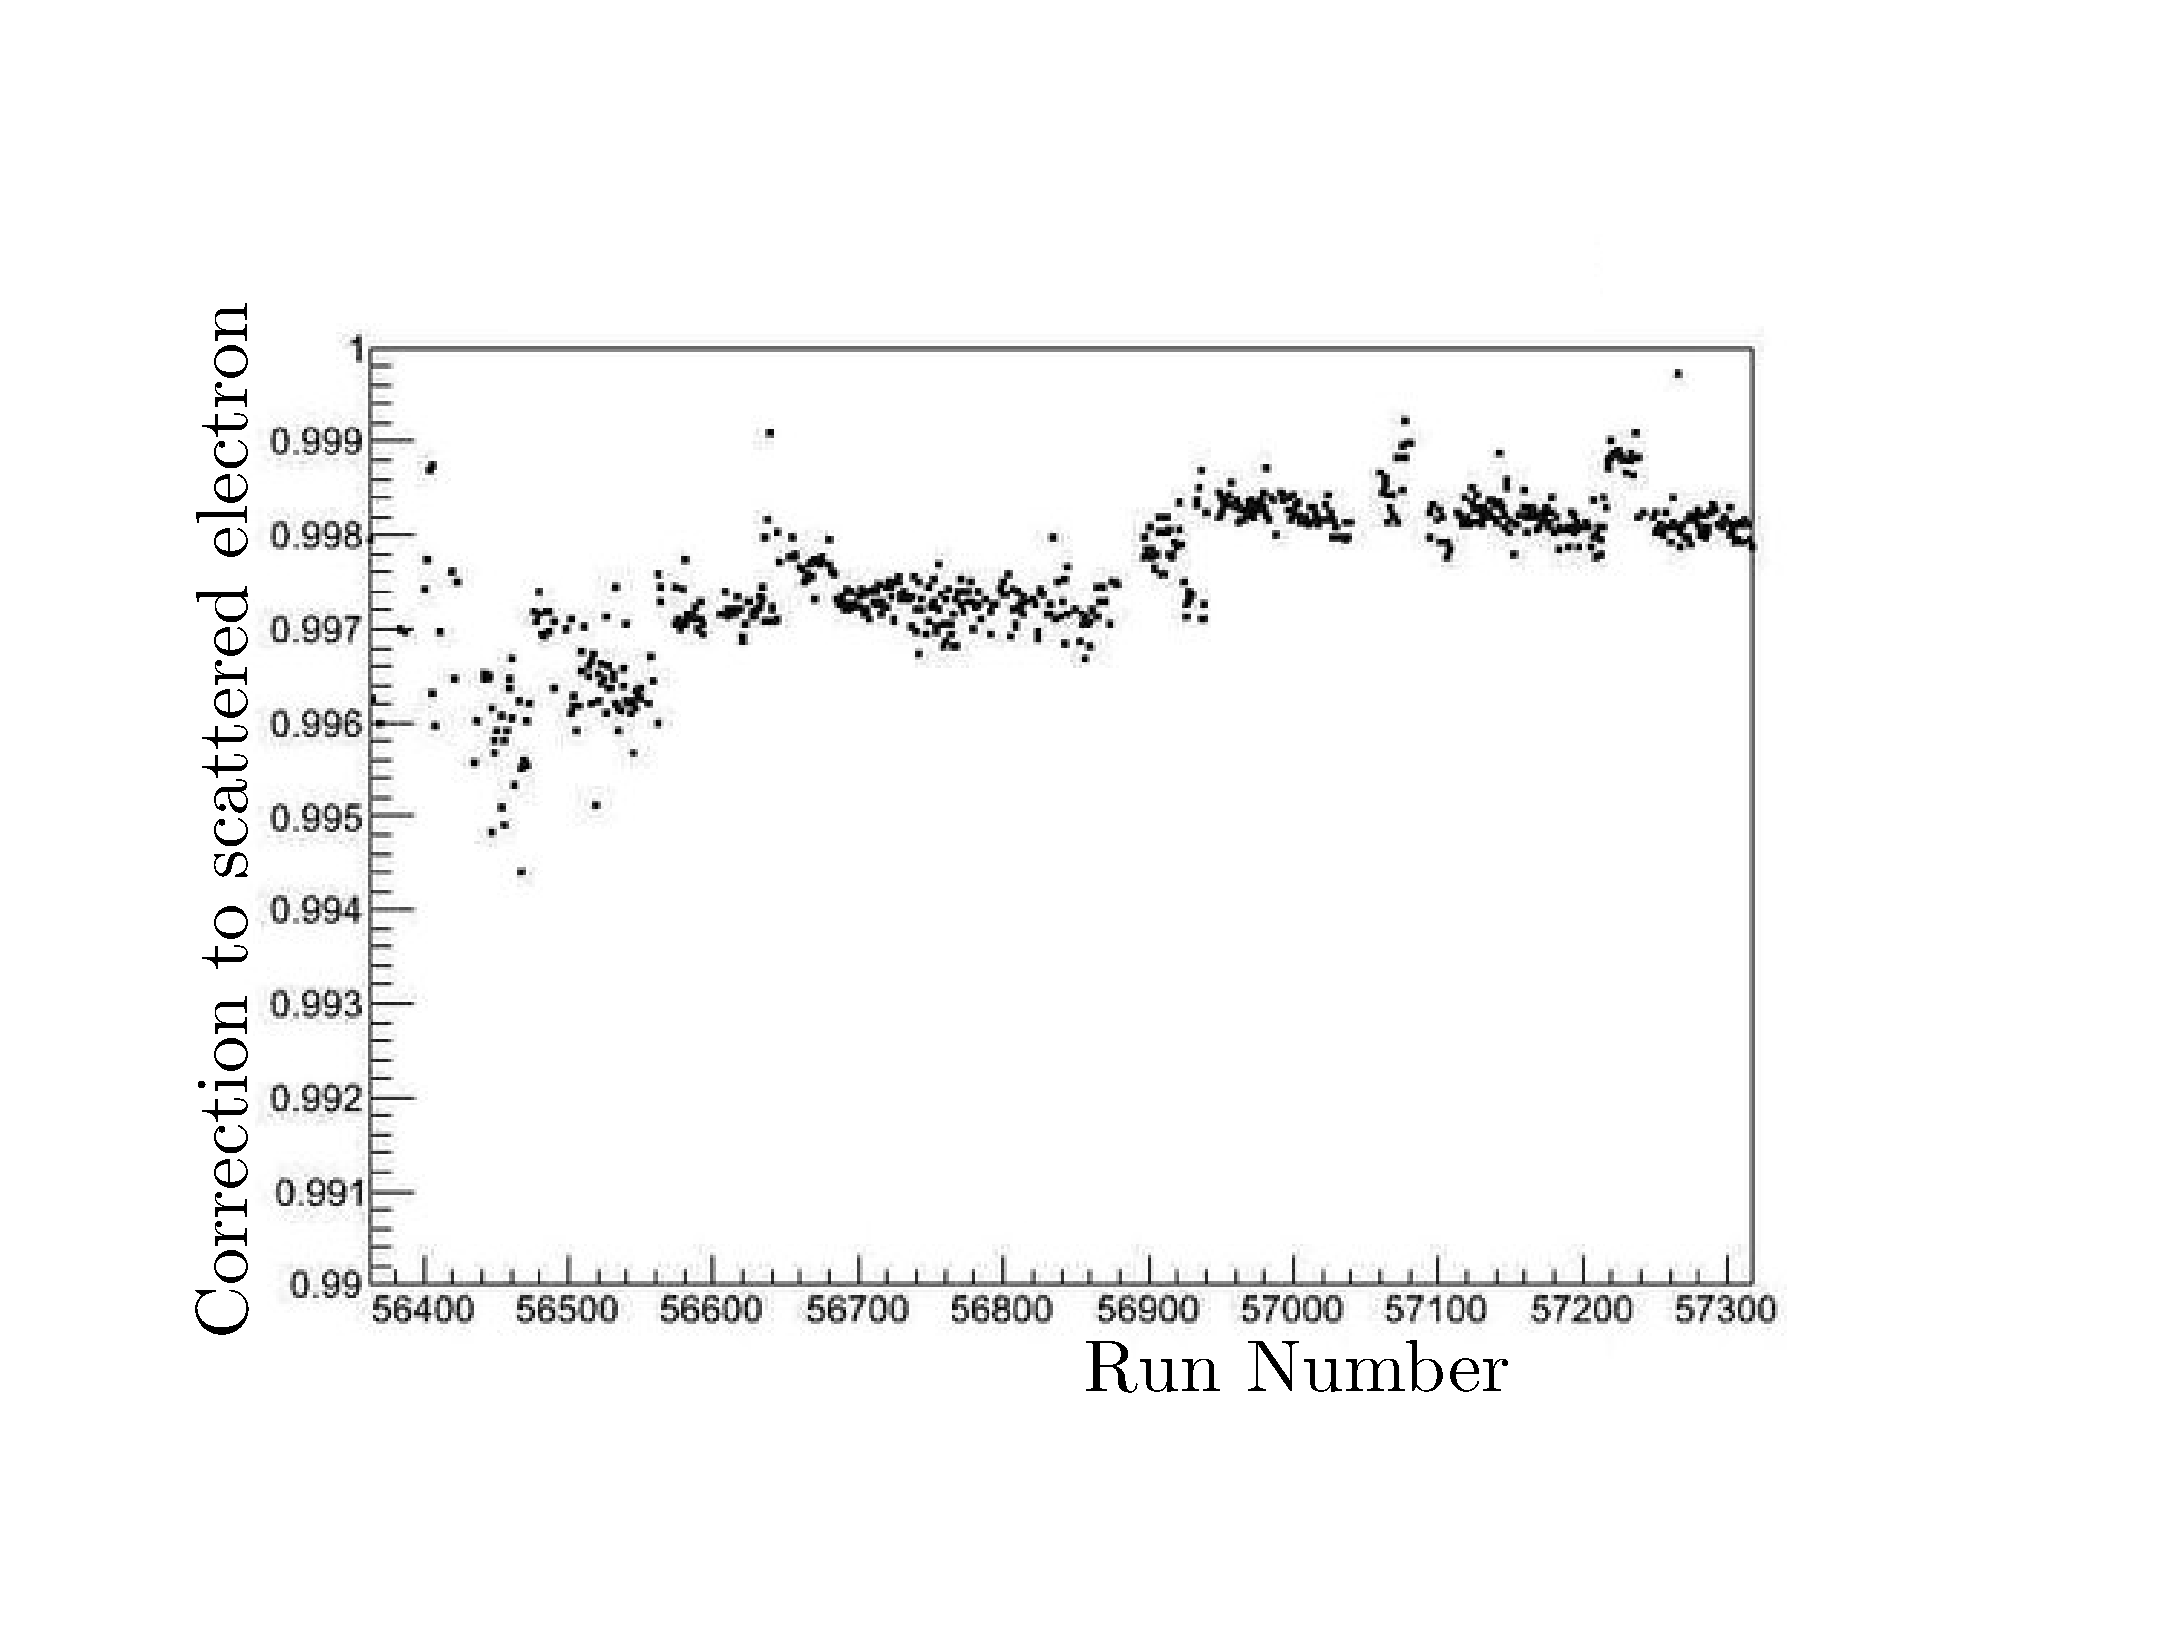
\includegraphics[width=0.6\textwidth]{figures/calib/tag/ecor/beam_cor.eps}
\caption[Beam Correction Factors for Entire \desg{g12} Runs]{\label{fig:beamcor.run} Plot of correction factor calculated for the entire \desg{g12} run set. Image source:~\cite{clas.thesis.kunkel}}
\end{center}\end{figure}

\begin{figure}\begin{center}
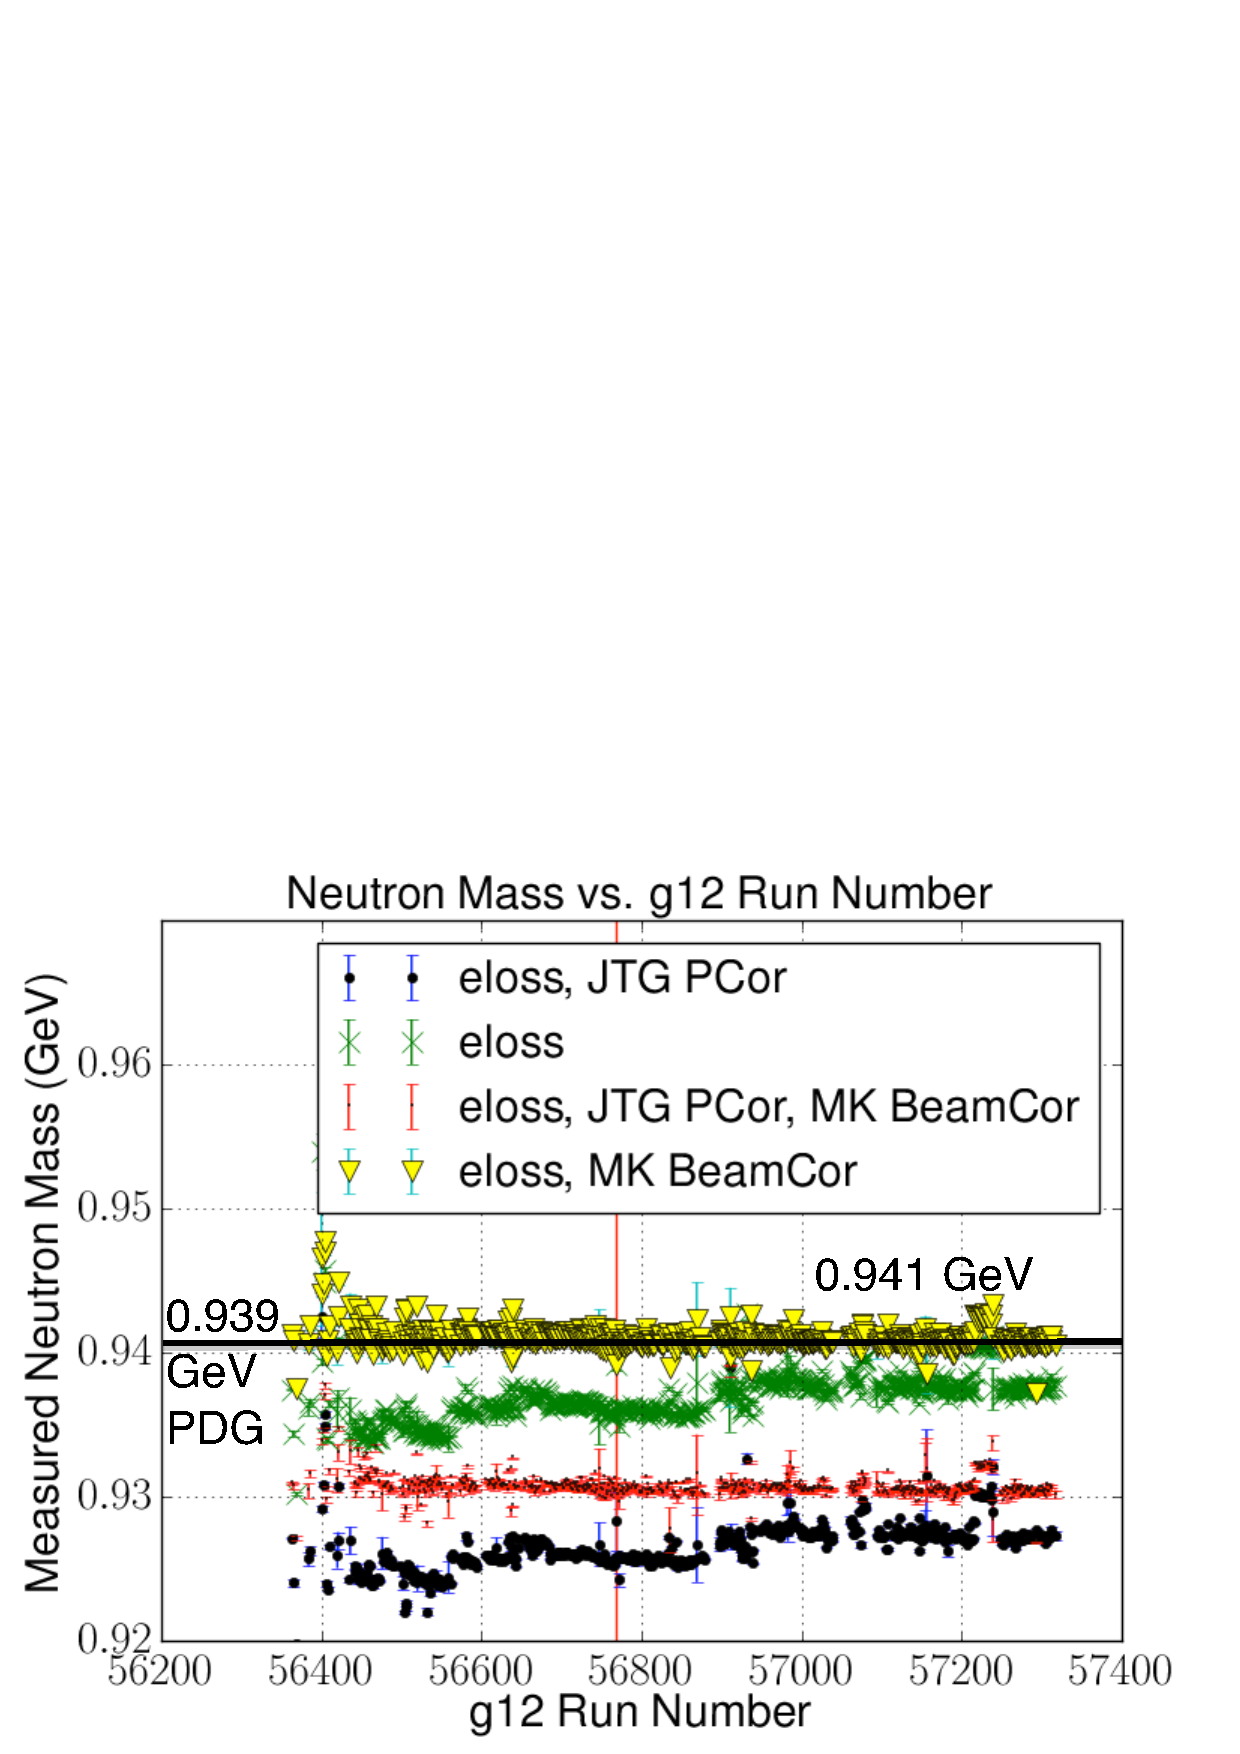
\includegraphics[width=0.6\textwidth]{figures/calib/tag/ecor/C3pi_allcorr_neutron_rxr.pdf}
\caption[Corrected Missing Neutron Mass for \desg{g12} Using Beam Corrections]{\label{fig:neutron.fixall} Plot of missing neutron mass using various corrections. The yellow triangles show a missing neutron mass with only ``energy-loss'' and beam correction applied (MK BeamCor) in which was the only corrections needed to correct the \desg{g12} data stream. \abbr{PDG} mass for the neutron is 0.939565 GeV/c.}
\end{center}\end{figure}



To correct for run by run shifts in the beam energy, use the header file in:
\begin{verbatim}
https://jlabsvn.jlab.org/svnroot/clas/trunk/analysis/g12/g12_ecor.hpp
\end{verbatim}

In the analysis program, the user needs to have the run number of the event and the uncorrected beam energy, then use:
\begin{verbatim}
corrected_beam_energy(int run, double uncorrected_beam_energy)
\end{verbatim}


\FloatBarrier
